\begin{filecontents*}{example.eps}
gsave
newpath
  20 20 moveto
  20 220 lineto
  220 220 lineto
  220 20 lineto
closepath
2 setlinewidth
gsave
  .4 setgray fill
grestore
stroke
grestore
\end{filecontents*}
\RequirePackage{fix-cm}
\documentclass[smallextended]{svjour3}       \smartqed  
\usepackage{xfrac}   
\usepackage{lineno}  
\usepackage{graphicx}
\usepackage{color}
\usepackage{multirow}
\usepackage{array}
\usepackage{setspace} 
\usepackage{makecell}
\usepackage{amsmath}

\newcolumntype{C}[1]{>{\centering\let\newline\\\arraybackslash\hspace{0pt}}m{#1}}

\renewcommand{\figurename}{Suppl. Fig.}
\renewcommand{\tablename}{Suppl. Table}


\linenumbers
\doublespacing 
\journalname{Molecular Breeding}
\begin{document}

\title{
Marker imputation efficiency for Genotyping-By-Sequencing data of crop species with and without a reference genome 
\thanks{Nelson Nazzicari and Filippo Biscarini contributed equally to the work \\
Corresponding author: Nelson Nazzicari \email{nelson.nazzicari@crea.gov.it}}
}

\titlerunning{Imputation efficiency for GBS data with and without the reference genome}        

\author{Nelson Nazzicari \and
  Filippo Biscarini  \and
  Paolo Cozzi \and
  E. Charles Brummer \and
  Paolo Annicchiarico
}

\authorrunning{Nazzicari, Biscarini et al.} 
\institute{
    N. Nazzicari, P. Annicchiarico \at Council for Agricultural Research and Economics (CREA) Research Centre for Fodder Crops and Dairy Productions, Lodi (Italy)
\and
    F. Biscarini, P. Cozzi \at Dipartimento di Bioinformatica, Fondazione Parco Tecnologico Padano, Lodi (Italy)
\and
    E.C. Brummer \at University of California, Plant Sciences Department, Davis, CA (USA)
}


\date{Received:  / Accepted:}

\maketitle

\graphicspath{{./figures/}}
\makeatletter{}\section{Supplementary material}
\label{sec:supplementary_material}

\subsection{SNP calling thresholds}
\label{sec:SNP_calling_thresholds}
Genotype calling can incur in two types of error, namely a heterozygote wrongly identified as homozigote ($HET \rightarrow HOM$) and the reverse case ($HOM \rightarrow HET$). 
Under the simplifying hypothesis of absence of sequencing errors and homogeneous sequencing quality, it is possible to estimate error rates for a tetraploid genome using the following formula:

\begin{equation}
\begin{cases}
0.75^{N_h} + 0.25^{N_h} & HET_{3-1} \rightarrow HOM \\ 
2 \times 0.5^{N_h}      & HET_{2-2} \rightarrow HOM \\ 
0                       & HOM \rightarrow HET
\end{cases}
\end{equation}

Where $N_h$ is the minimum number of reads required to label a stack of aligning reads as heterozygote. The discussed case of $N_h = 11$ brings to a total expected $HET \rightarrow HOM$ error rate of 4.22\%.\\
The hypothesis mentioned above greatly simplyfies the real case (e.g. $HOM \rightarrow HET$ errors can not happen, since a homozigote will always produce 100\% of reads of the same type). When accounting sequencing errors and reads quality a term for $HOM \rightarrow HET$ appears, due to reads sequenced as the wrong allele. In the presented study we thus applied a threshold of 4 required reads per stack to call a homozigote to minimize this kind of error.

\subsection{Supplementary tables}
\label{sec:supplementary_tables}
\makeatletter{}\begin{table}
\centering
\caption[Accuracy statistics]{Imputation accuracies (as percentages) for the various
datasets and methods, averaged over all allowed and injected missing thresholds. Rice data are reported averaged by chromosome and on the complete genotypes. Alfalfa data are reported averaged over the two Alfalfa-PV and Alfalfa-Med populations. FILLIN failed to impute alfalfa datasets.}
\label{tab:accuracy_statistics}
\begin{tabular}{llcccc}
\hline\noalign{\smallskip}
\noalign{\smallskip}\hline\noalign{\smallskip}
\textbf{Dataset} & \textbf{Method} & \textbf{Total} & \textbf{Minor (BB)} & \textbf{Major (AA)} & \textbf{Heterozygote (AB)}\\
\noalign{\smallskip}\Xhline{3\arrayrulewidth}\noalign{\smallskip}
alfalfa & Beagle & 73.14 & 14.27 & 99.37 & 20.77\\
alfalfa & Beagle (shuffle) & 66.34 & 1.31 & 99.88 & 0.50\\
alfalfa & kNNI & 82.20 & 14.68 & 90.82 & 66.03\\
alfalfa & MNI & 78.38 & 0.00 & 88.69 & 58.88\\
alfalfa & RFI  & 79.50 & 0.01 & 89.05 & 61.75\\
alfalfa & SVDI & 77.36 & 4.47 & 85.81 & 61.67\\
alfalfa & FILLIN & * & * & * & *\\
alfalfa & FILLIN (shuffle)  & * & * & * & *\\
rice (chr) & Beagle & 99.58 & 97.50 & 99.80 & -\\
rice (chr) & Beagle (shuffle) & 96.09 & 74.73 & 98.42 & -\\
rice (chr) & kNNI & 98.10 & 89.12 & 99.04 & -\\
rice (chr) & MNI & 90.19 & 1.06 & 99.89 & -\\
rice (chr) & RFI  & 98.81 & 91.51 & 99.58 & -\\
rice (chr) & SVDI & 97.81 & 85.64 & 99.11 & -\\
rice (chr) & FILLIN & 86.96 & 63.62 & 90.14 & -\\
rice (chr) & FILLIN (shuffle)  & 82.19 & 55.86 & 85.81 & -\\
rice & Beagle & 99.58 & 97.57 & 99.80 & -\\
rice & Beagle (shuffle) & 93.48 & 55.64 & 97.69 & -\\
rice & kNNI & 98.30 & 89.80 & 99.19 & -\\
rice & MNI & 90.21 & 0.61 & 99.89 & -\\
rice & RFI  & 97.86 & 84.68 & 99.28 & -\\
rice & SVDI & 95.74 & 70.96 & 98.40 & -\\
\noalign{\smallskip}\hline
\end{tabular}
\end{table}



 

\subsection{Supplementary figures}
\label{sec:supplementary_figures}

\begin{figure}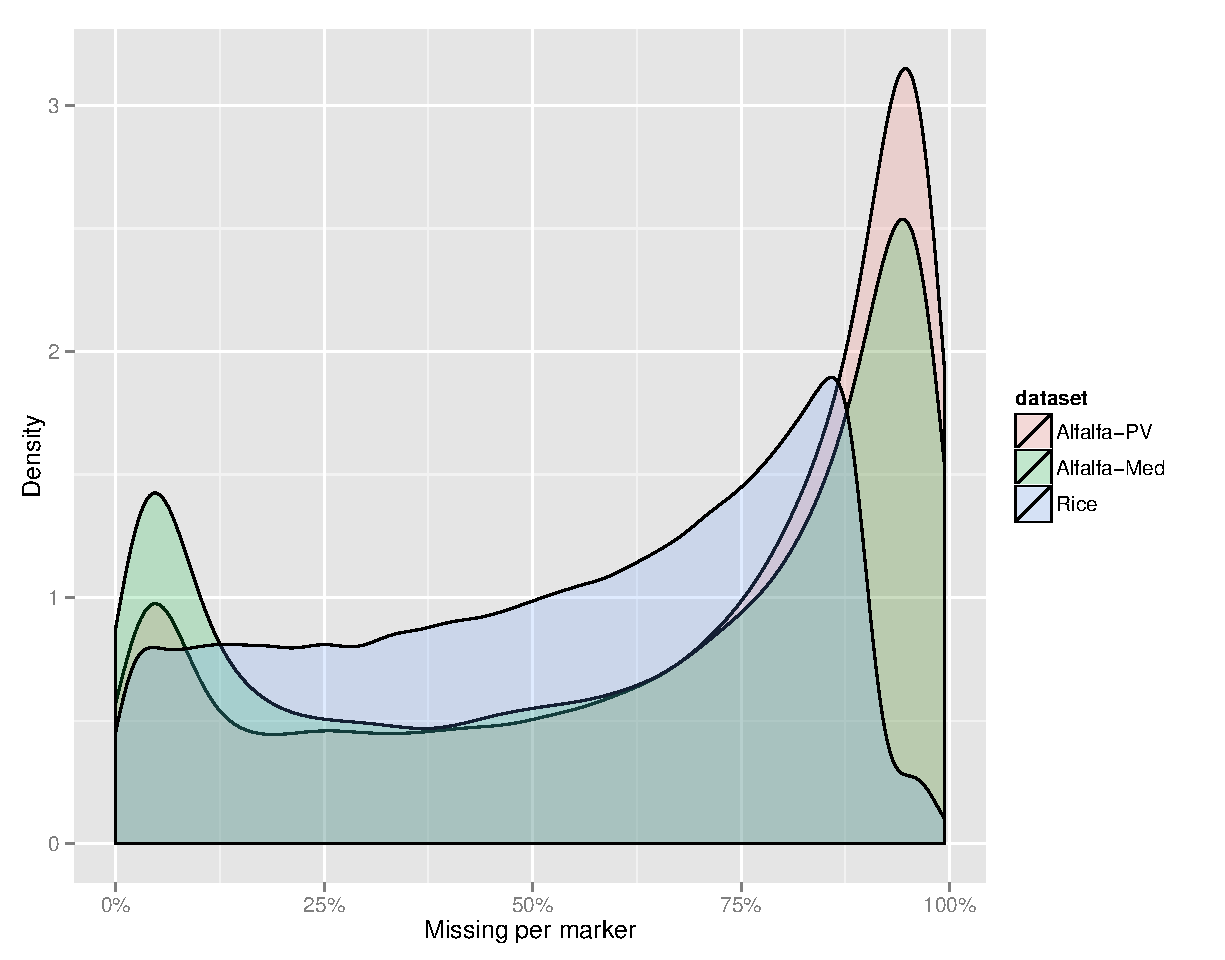
\includegraphics[width=0.95\textwidth]{SupplFig01_miss_per_marker.pdf}
\caption{Distribution of missings-per-marker rates in the three datasets. This is a
density plot, so all curves delimit the same unitary area.}
\end{figure}

\begin{figure}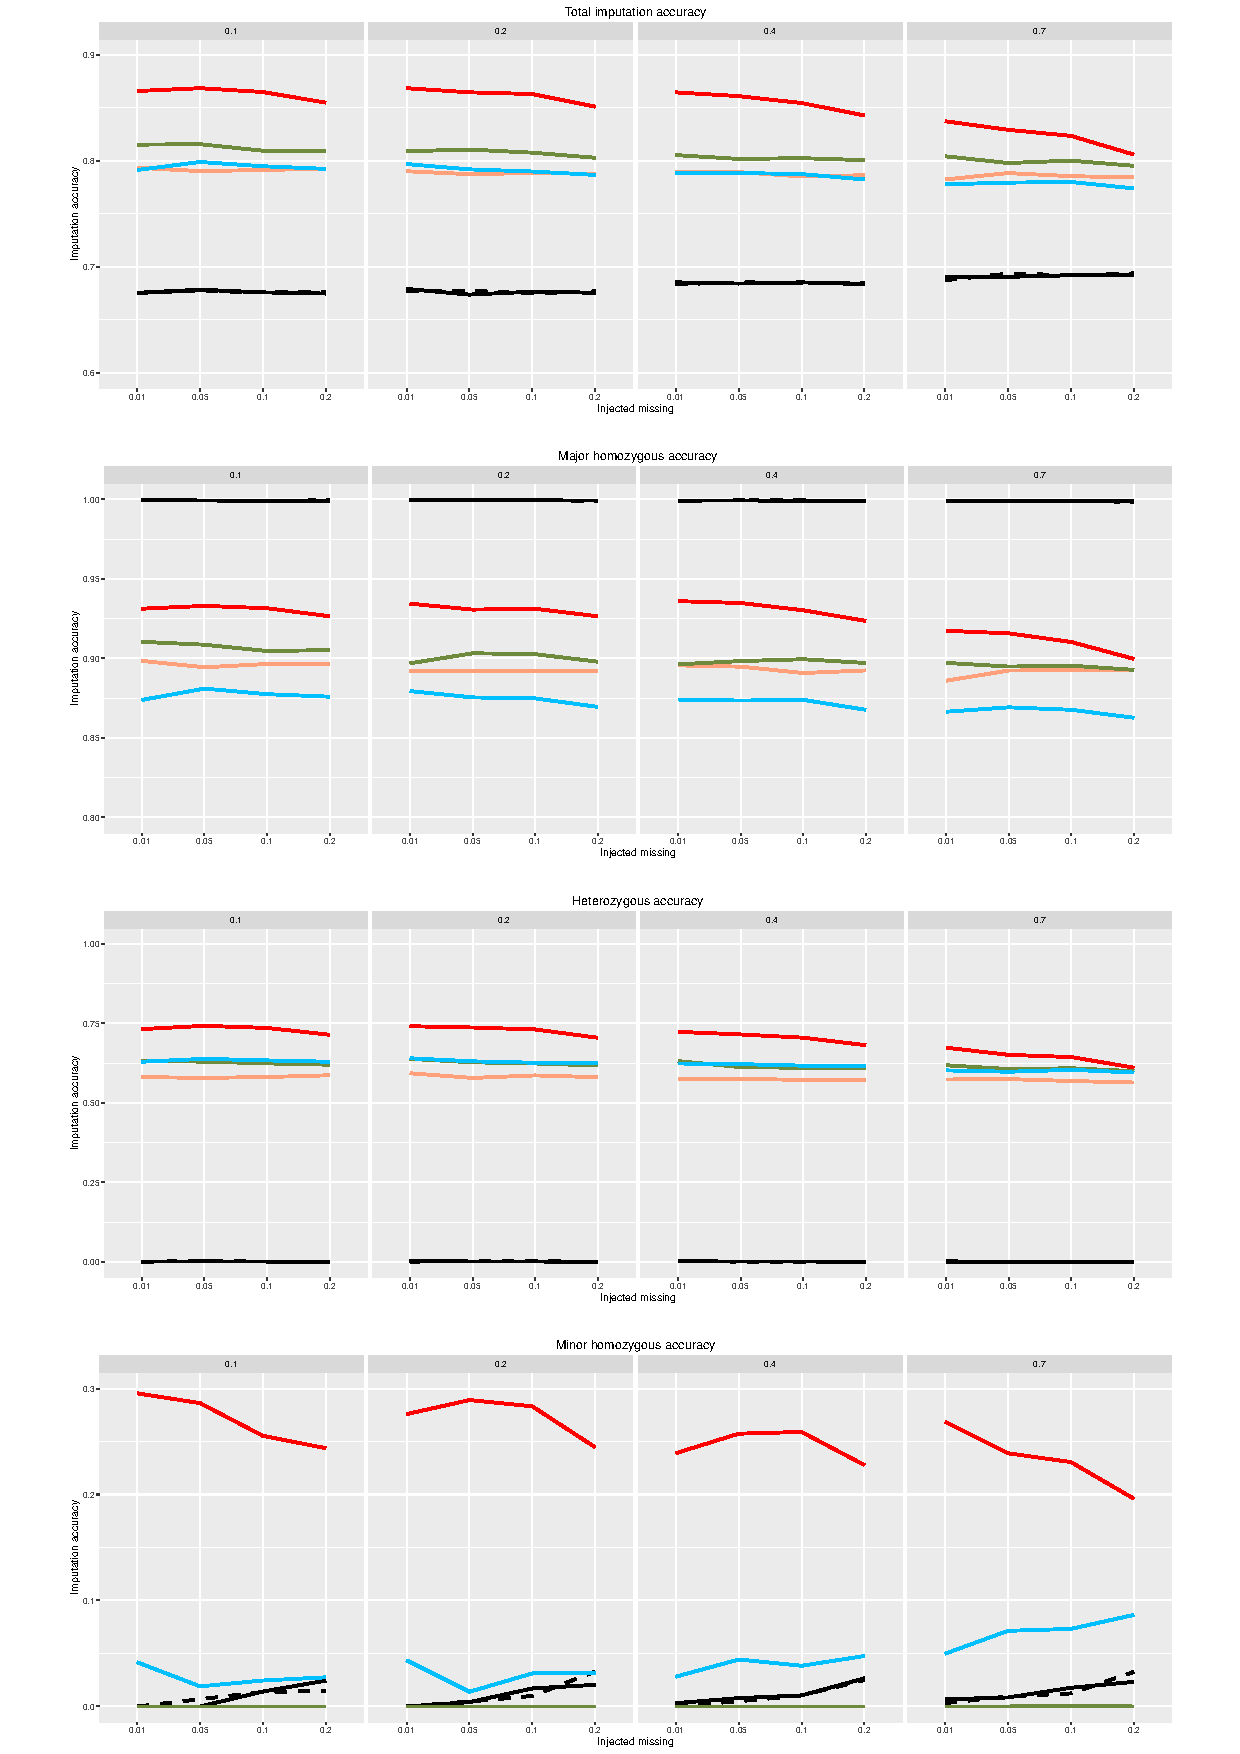
\includegraphics[width=0.95\textwidth]{figure_reforma.pdf}\caption{
imputation accuracies overall, for the major homozygous genotype (AA), for heterozygotes (AB), and for the minor homozygous genotype (BB) in datasets consisting of
10\%, 20\%, 40\% and 70\% allowed missing data per locus (boxes) with 1\%, 5\%, 10\% and 20\%
additional missing values artificially introduced (x-axis) for alfalfa population Alfalfa-Med.
Lines colors represent the five imputation algorithms: MNI (salmon), KNNI (red), SVDI (blue), RFI (green), Beagle with ordered markers (solid black) and Beagle with unordered markers (dashed black)}\end{figure}

\begin{figure}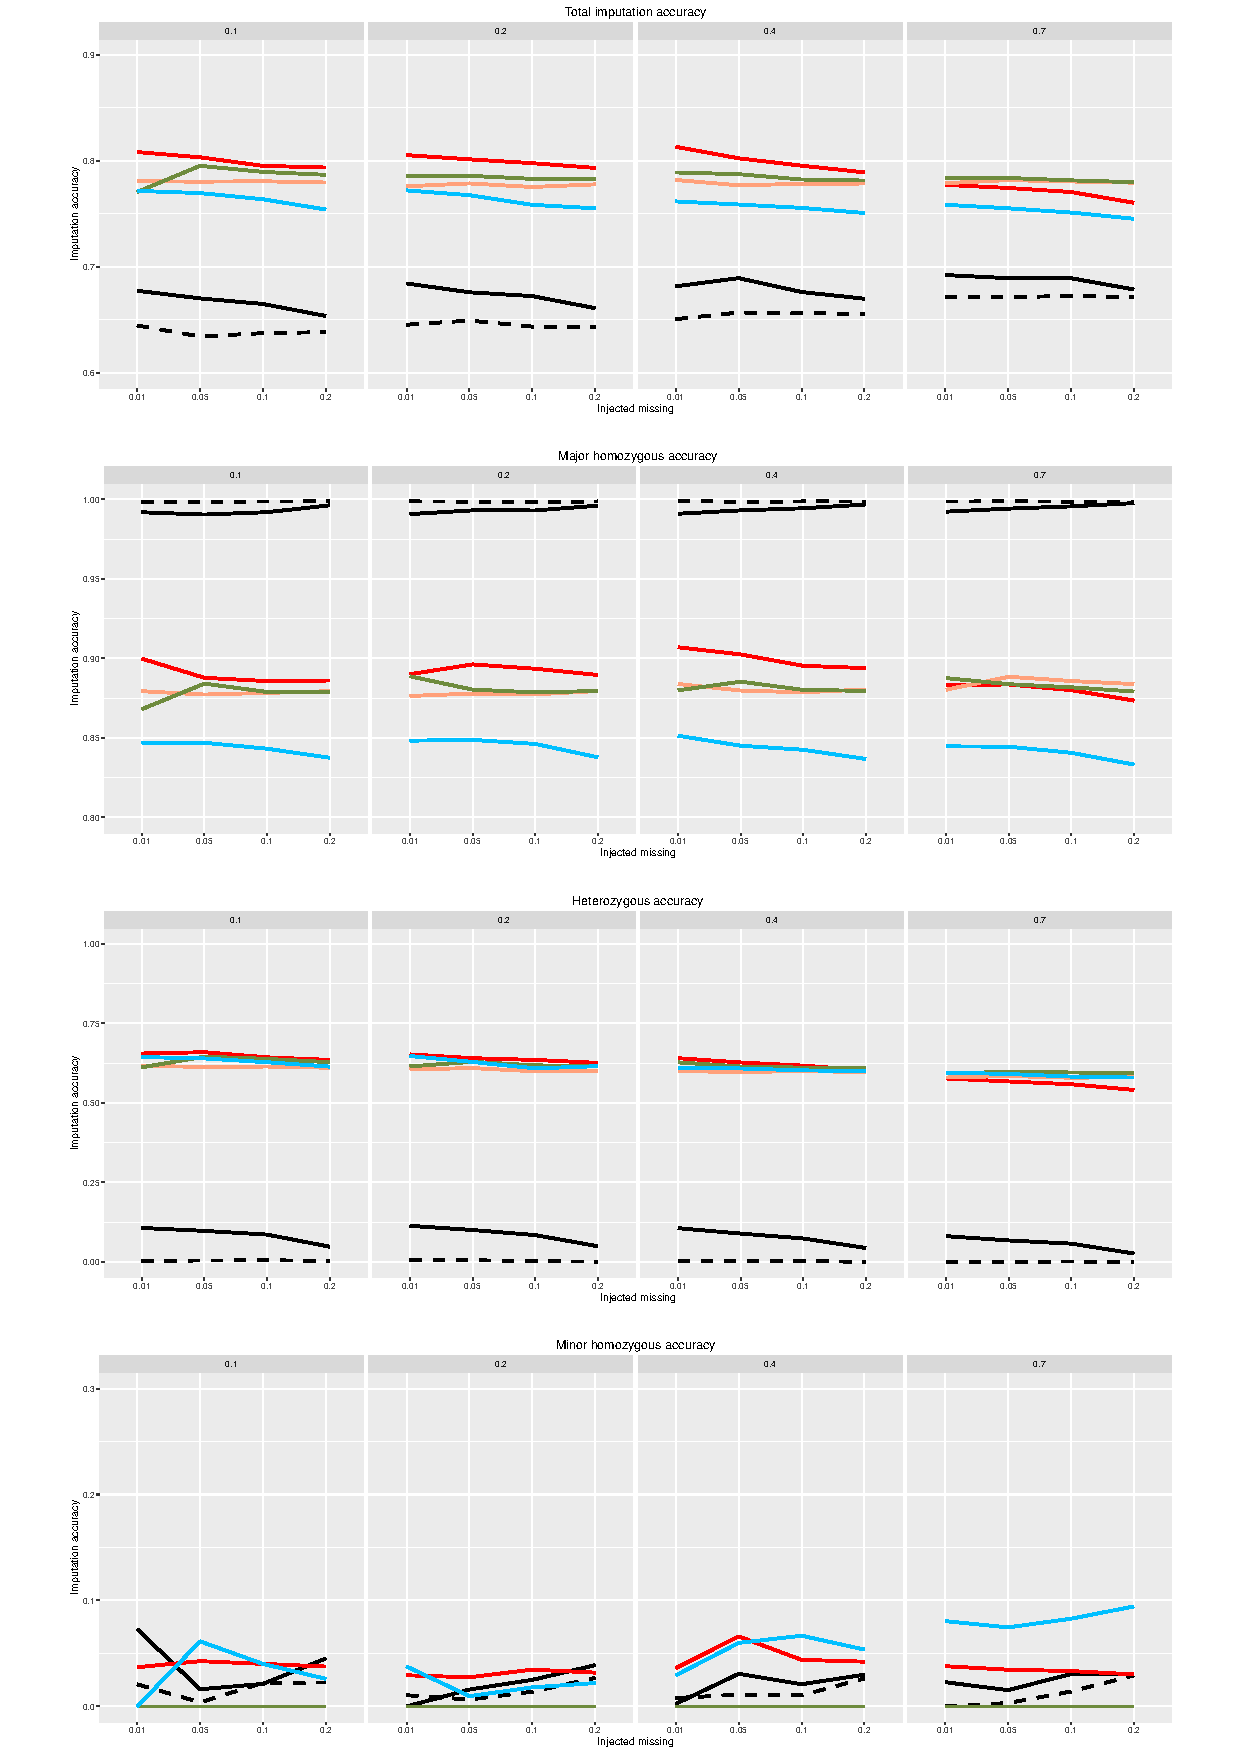
\includegraphics[width=0.95\textwidth]{figure_lodi.pdf}\caption{
imputation accuracies overall, for the major homozygous genotype (AA), for heterozygotes (AB), and for the minor homozygous genotype (BB) in datasets consisting of
10\%, 20\%, 40\% and 70\% allowed missing data per locus (boxes) with 1\%, 5\%, 10\% and 20\%
additional missing values artificially introduced (x-axis) for alfalfa population Alfalfa-PV.
Lines colors represent the five imputation algorithms: MNI (salmon), KNNI (red), SVDI (blue), RFI (green), Beagle with ordered markers (solid black) and Beagle with unordered markers (dashed black)}\end{figure}

\begin{figure}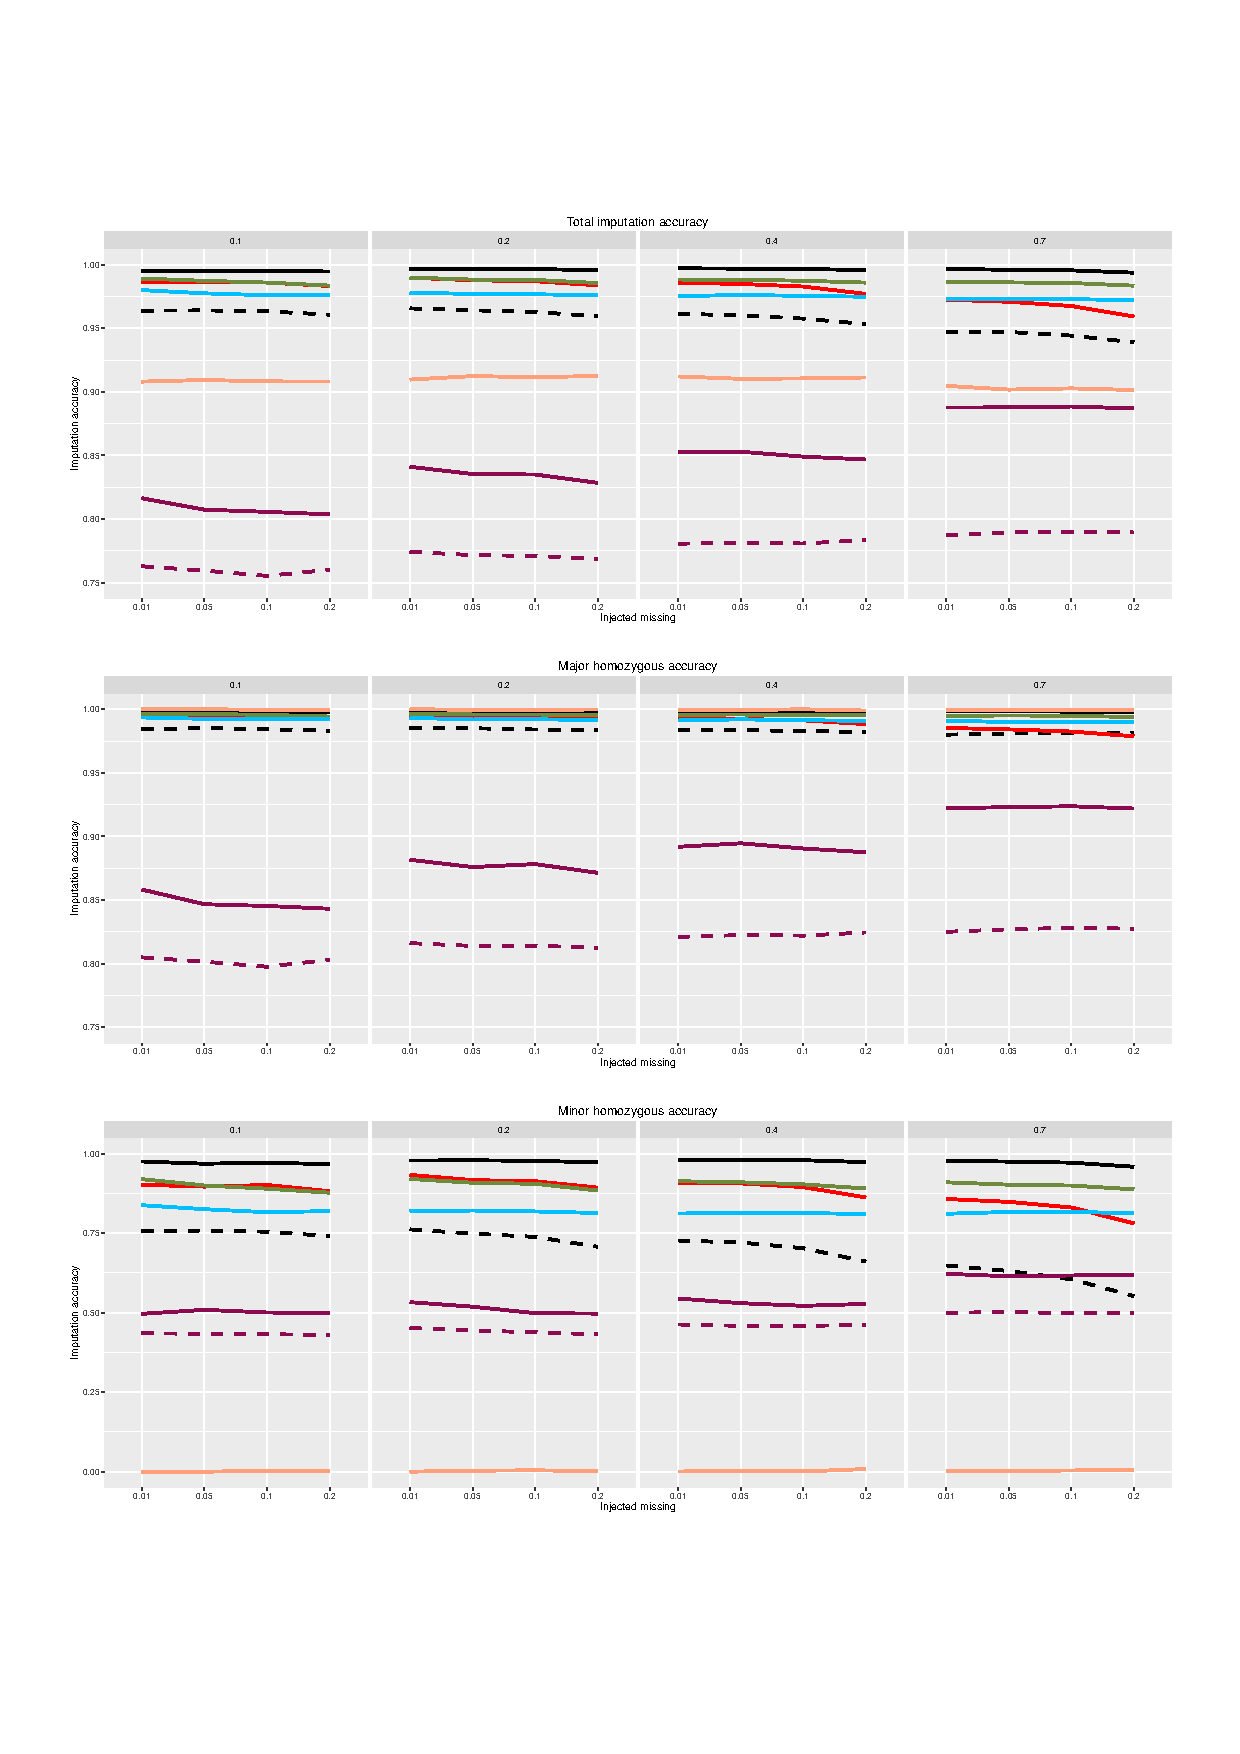
\includegraphics[width=0.95\textwidth]{figure_rice_chrom_1.pdf}\caption{
imputation accuracies overall, for the major homozygous genotype (AA) and for the minor homozygous genotype (BB) in datasets consisting of
10\%, 20\%, 40\% and 70\% allowed missing data per locus (boxes) with 1\%, 5\%, 10\% and 20\%
additional missing values artificially introduced (x-axis) for rice chromosome 1 data.
Lines colors represent the five imputation algorithms: MNI (salmon), KNNI (red), SVDI (blue), RFI (green), Beagle with ordered markers (solid black) and Beagle with unordered markers (dashed black)}\end{figure}

\begin{figure}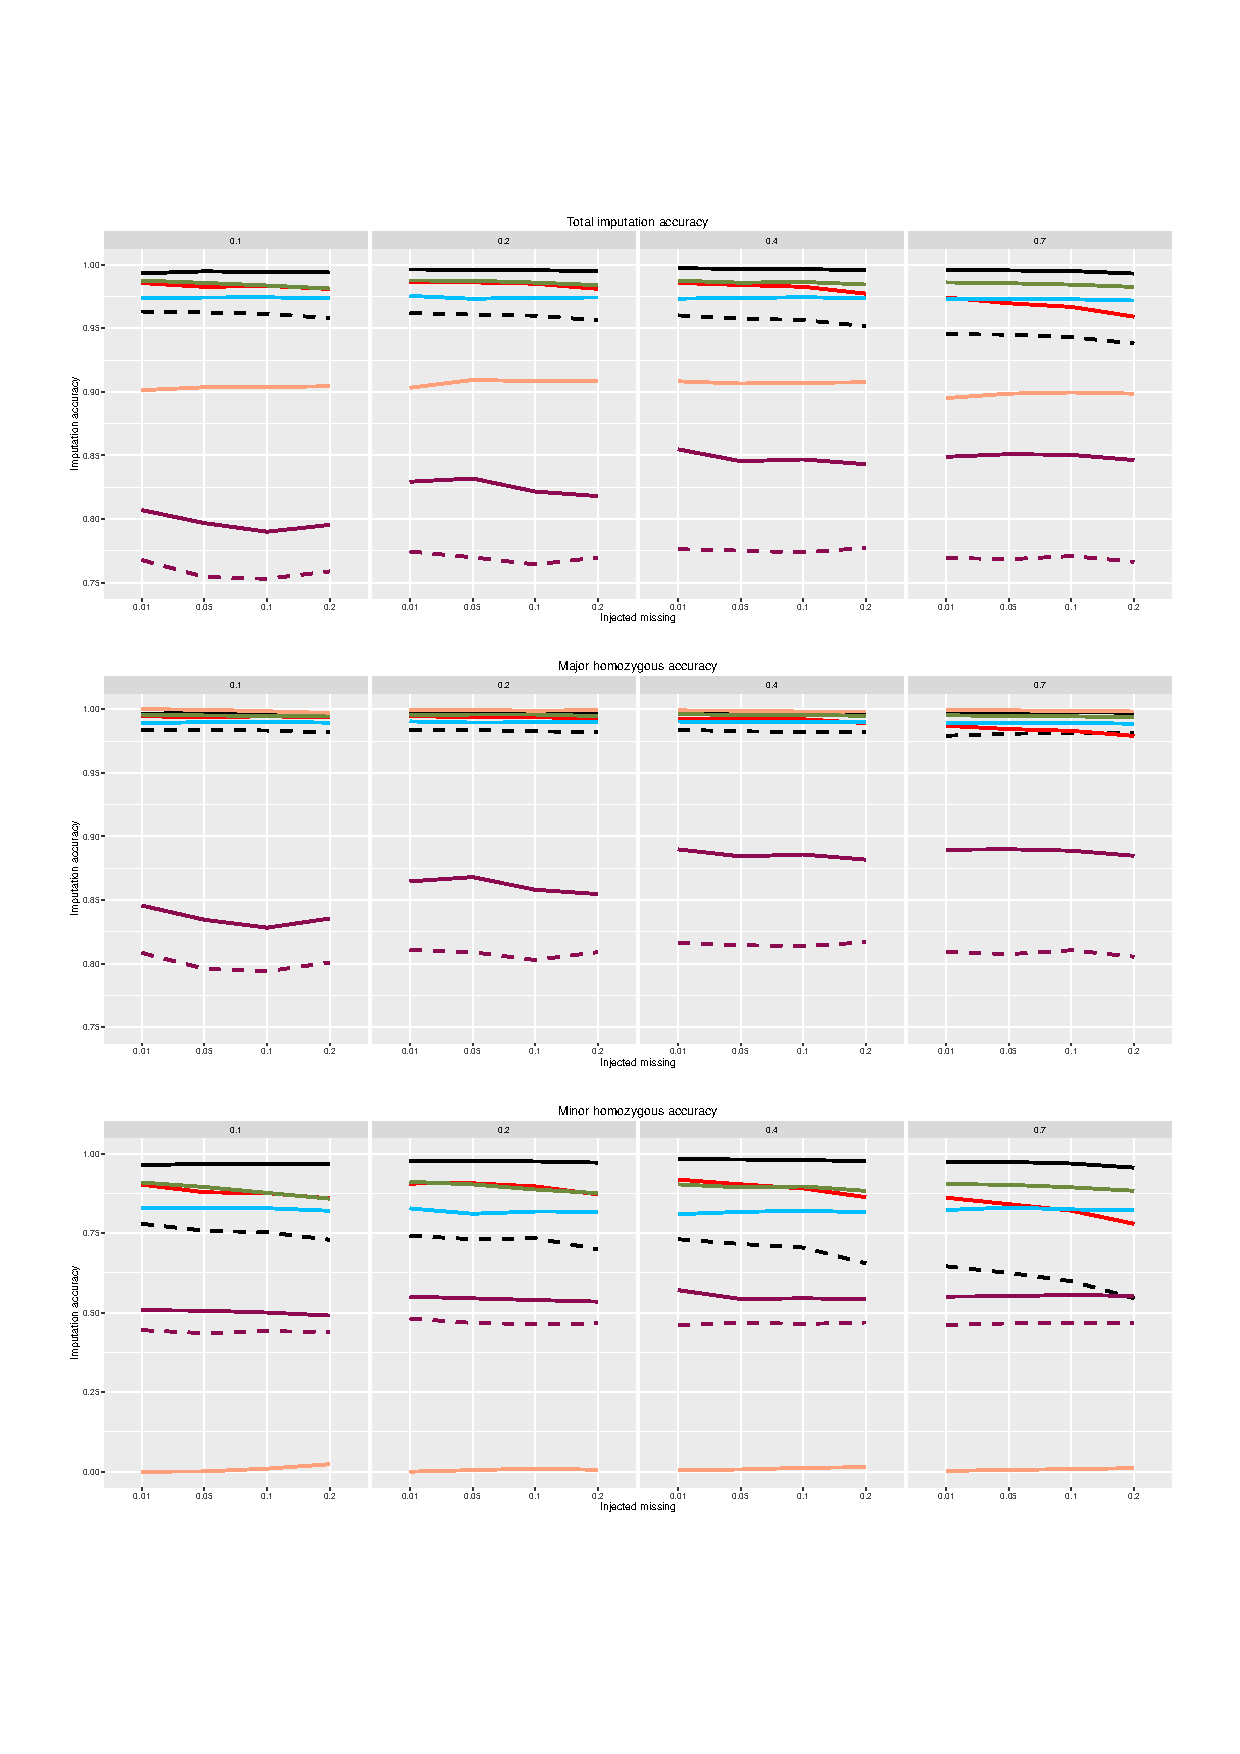
\includegraphics[width=0.95\textwidth]{figure_rice_chrom_2.pdf}\caption{
imputation accuracies overall, for the major homozygous genotype (AA) and for the minor homozygous genotype (BB) in datasets consisting of
10\%, 20\%, 40\% and 70\% allowed missing data per locus (boxes) with 1\%, 5\%, 10\% and 20\%
additional missing values artificially introduced (x-axis) for rice chromosome 2 data.
Lines colors represent the five imputation algorithms: MNI (salmon), KNNI (red), SVDI (blue), RFI (green), Beagle with ordered markers (solid black) and Beagle with unordered markers (dashed black)}\end{figure}

\begin{figure}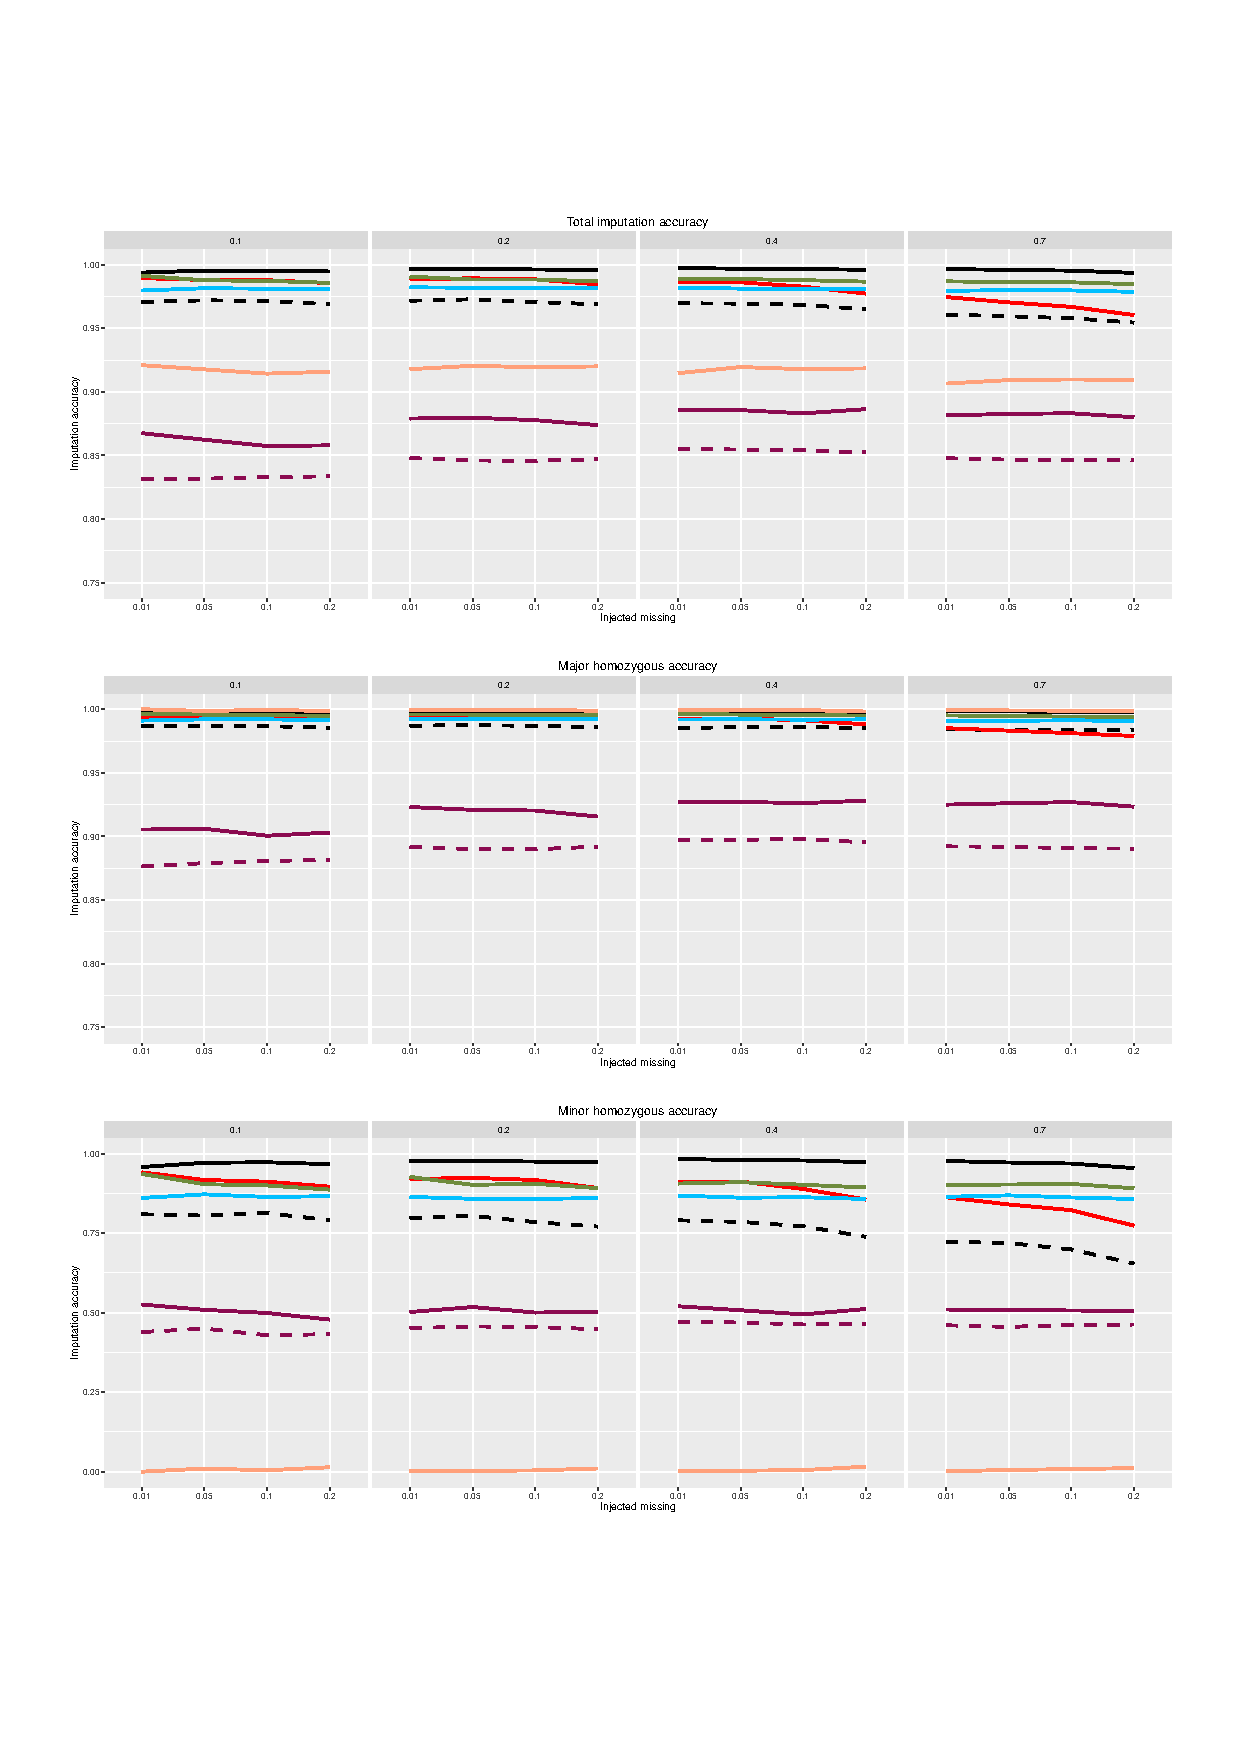
\includegraphics[width=0.95\textwidth]{figure_rice_chrom_3.pdf}\caption{
imputation accuracies overall, for the major homozygous genotype (AA) and for the minor homozygous genotype (BB) in datasets consisting of
10\%, 20\%, 40\% and 70\% allowed missing data per locus (boxes) with 1\%, 5\%, 10\% and 20\%
additional missing values artificially introduced (x-axis) for rice chromosome 3 data.
Lines colors represent the five imputation algorithms: MNI (salmon), KNNI (red), SVDI (blue), RFI (green), Beagle with ordered markers (solid black) and Beagle with unordered markers (dashed black)}\end{figure}

\begin{figure}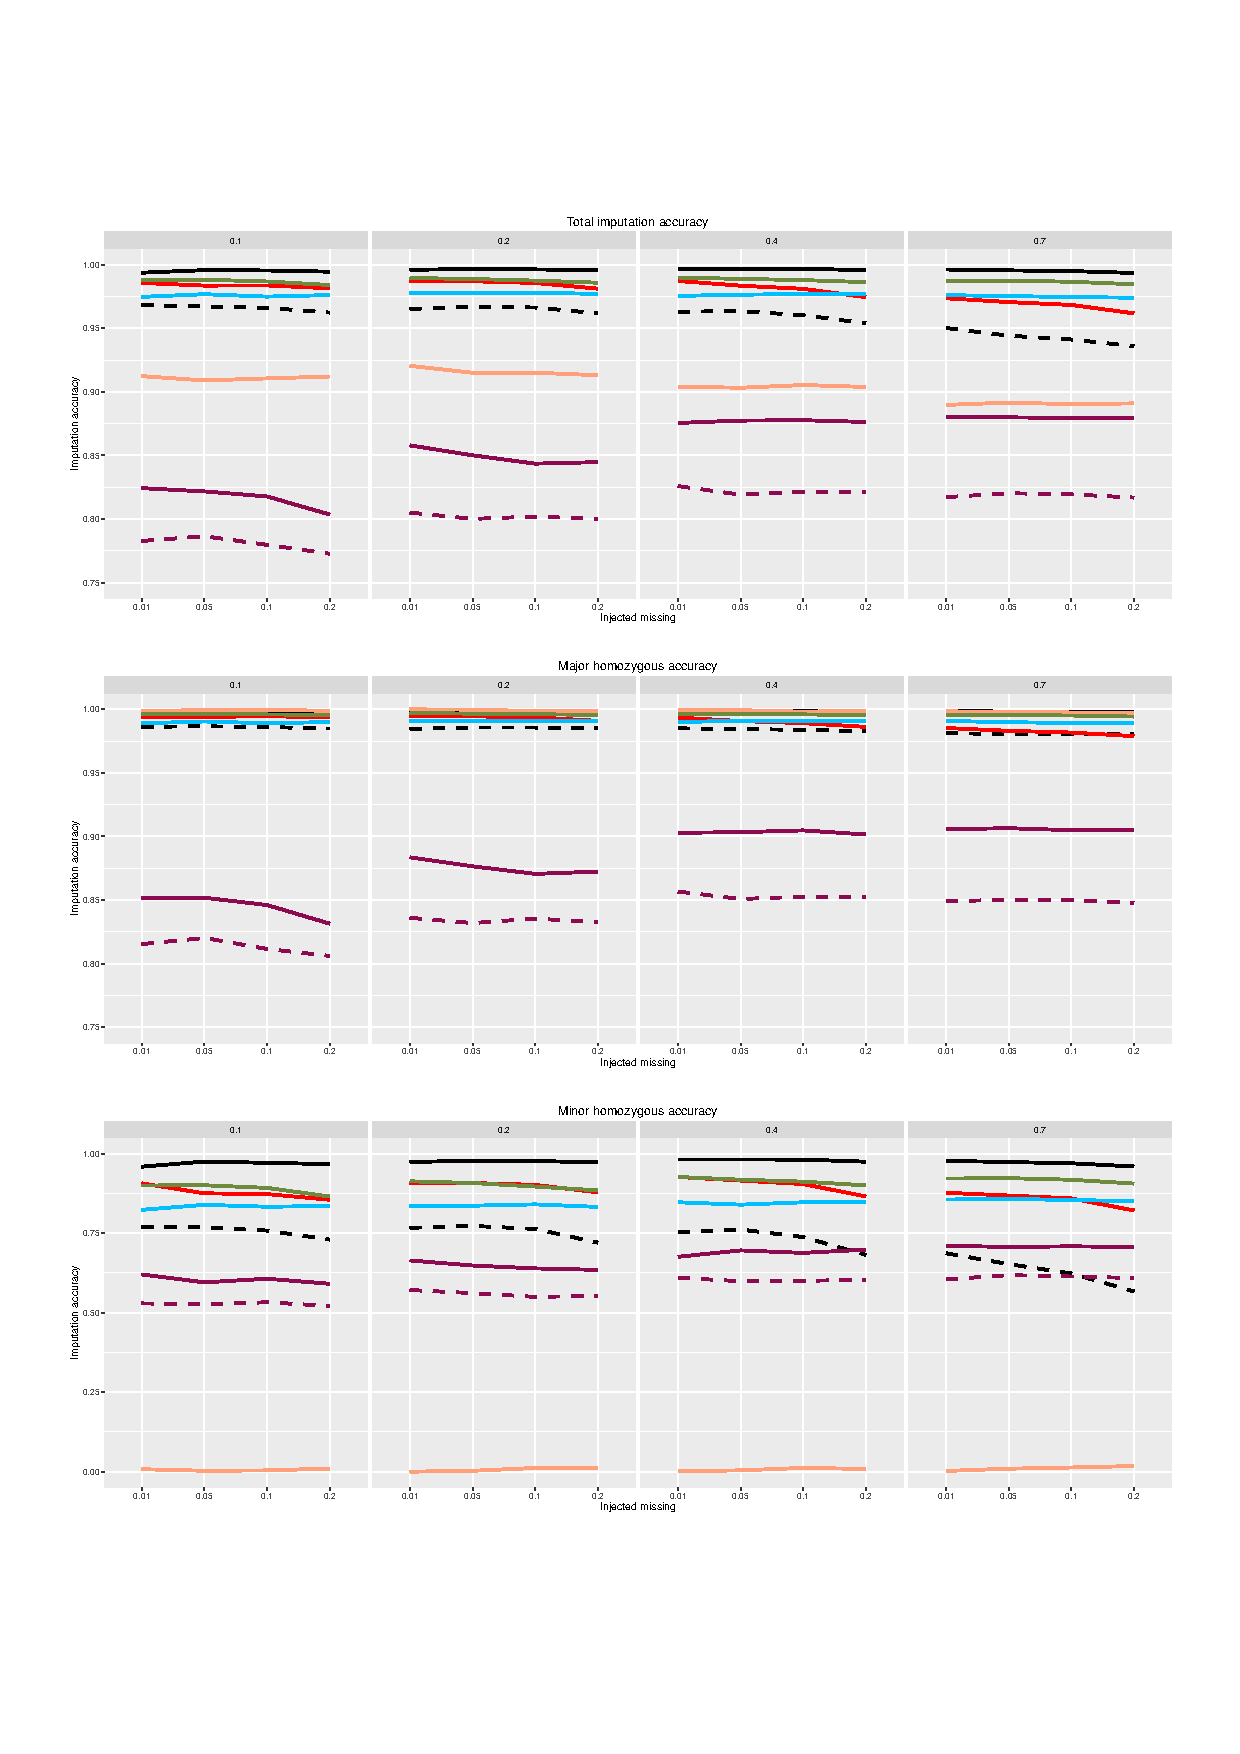
\includegraphics[width=0.95\textwidth]{figure_rice_chrom_4.pdf}\caption{
imputation accuracies overall, for the major homozygous genotype (AA) and for the minor homozygous genotype (BB) in datasets consisting of
10\%, 20\%, 40\% and 70\% allowed missing data per locus (boxes) with 1\%, 5\%, 10\% and 20\%
additional missing values artificially introduced (x-axis) for rice chromosome 4 data.
Lines colors represent the five imputation algorithms: MNI (salmon), KNNI (red), SVDI (blue), RFI (green), Beagle with ordered markers (solid black) and Beagle with unordered markers (dashed black)}\end{figure}

\begin{figure}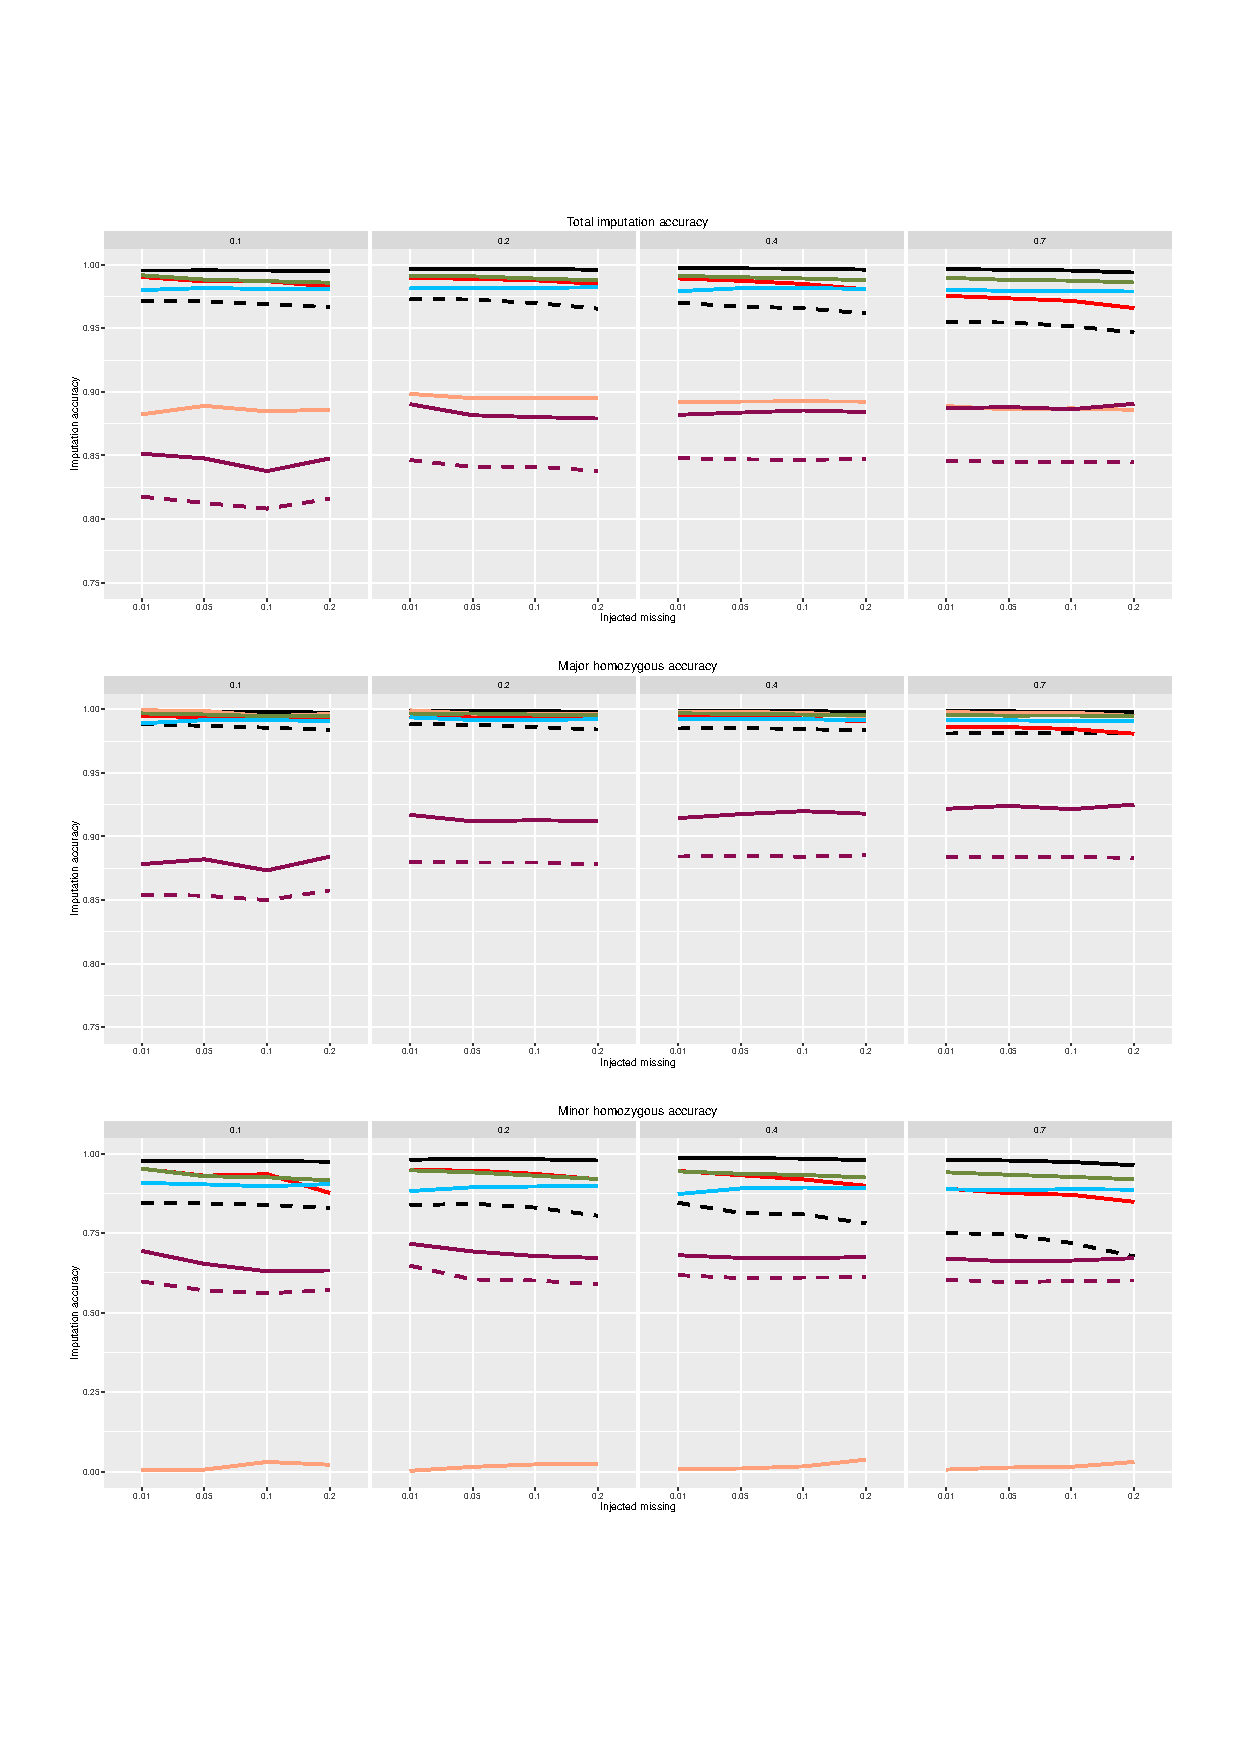
\includegraphics[width=0.95\textwidth]{figure_rice_chrom_5.pdf}\caption{
imputation accuracies overall, for the major homozygous genotype (AA) and for the minor homozygous genotype (BB) in datasets consisting of
10\%, 20\%, 40\% and 70\% allowed missing data per locus (boxes) with 1\%, 5\%, 10\% and 20\%
additional missing values artificially introduced (x-axis) for rice chromosome 5 data.
Lines colors represent the five imputation algorithms: MNI (salmon), KNNI (red), SVDI (blue), RFI (green), Beagle with ordered markers (solid black) and Beagle with unordered markers (dashed black)}\end{figure}

\begin{figure}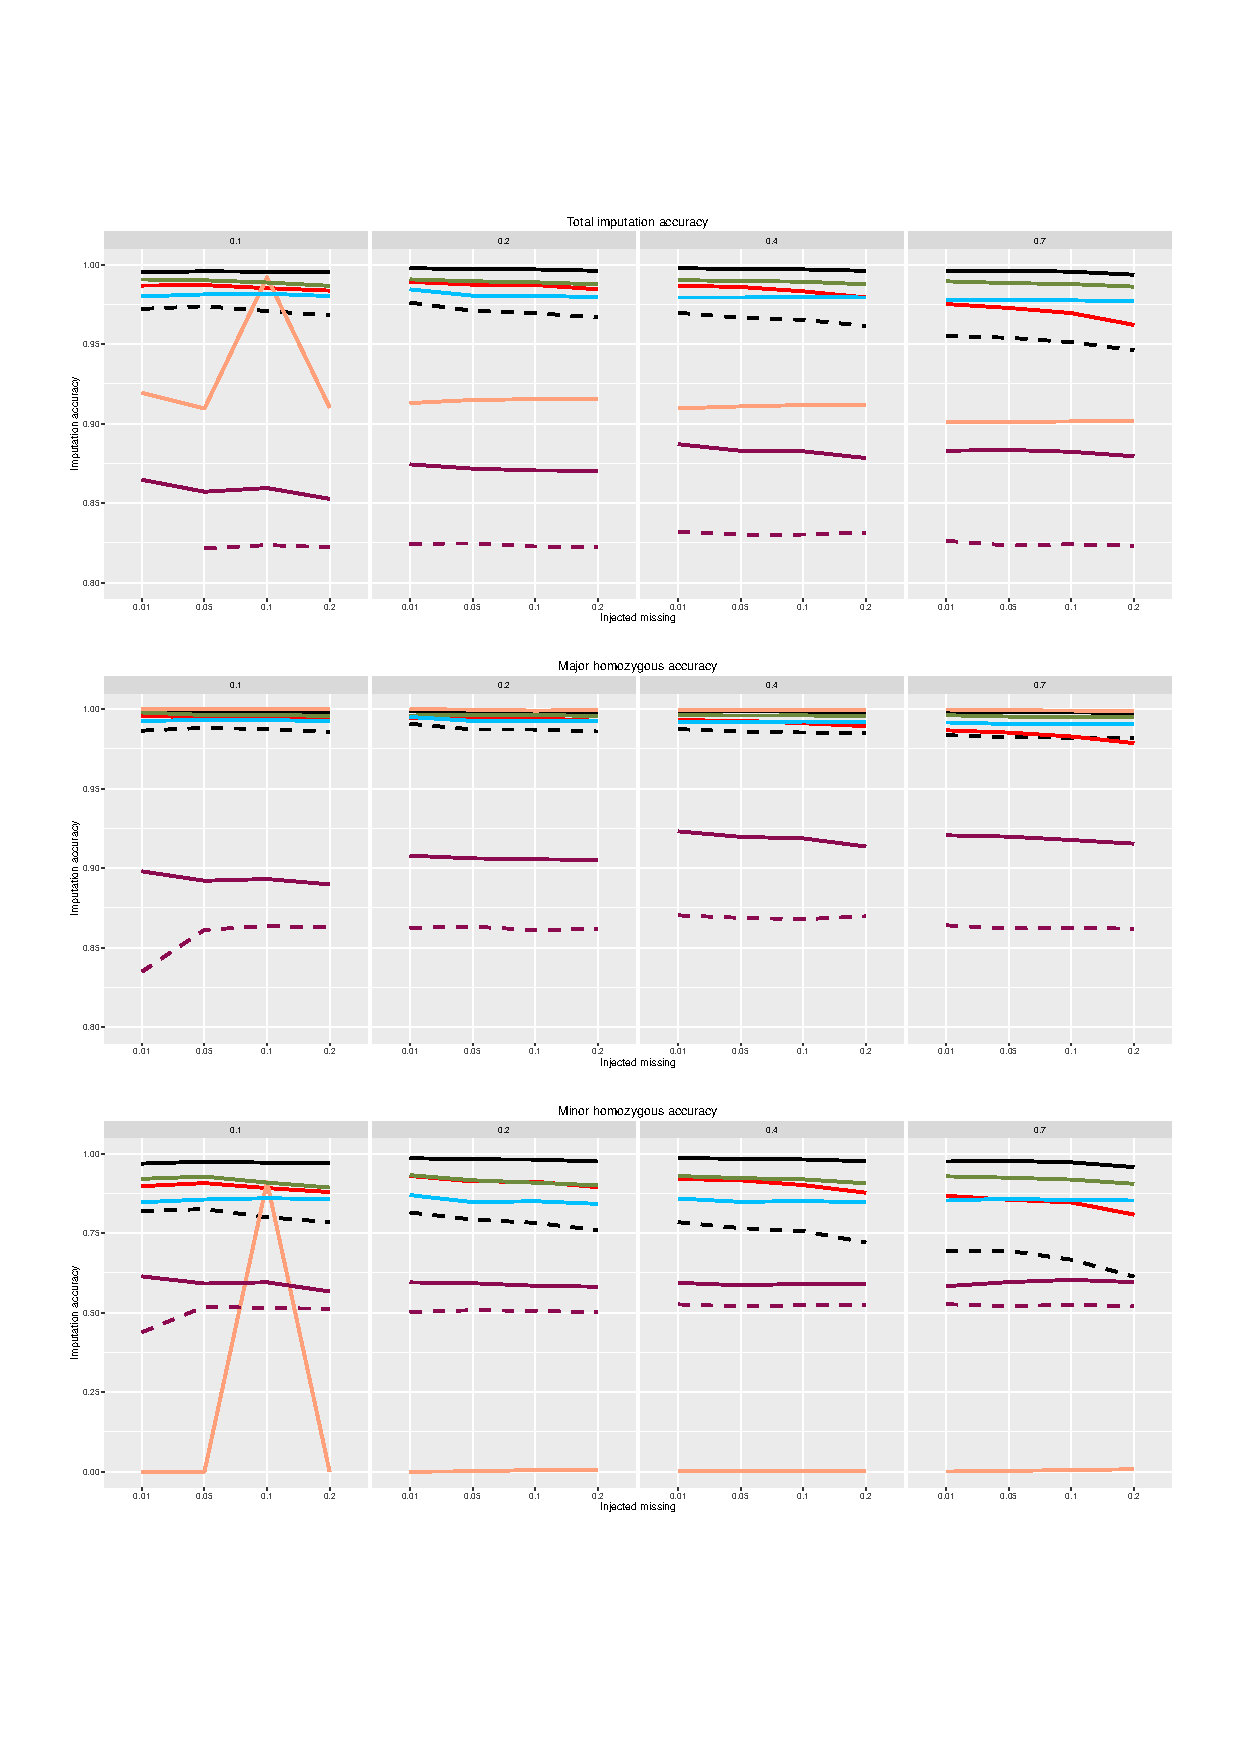
\includegraphics[width=0.95\textwidth]{figure_rice_chrom_6.pdf}\caption{
imputation accuracies overall, for the major homozygous genotype (AA) and for the minor homozygous genotype (BB) in datasets consisting of
10\%, 20\%, 40\% and 70\% allowed missing data per locus (boxes) with 1\%, 5\%, 10\% and 20\%
additional missing values artificially introduced (x-axis) for rice chromosome 6 data.
Lines colors represent the five imputation algorithms: MNI (salmon), KNNI (red), SVDI (blue), RFI (green), Beagle with ordered markers (solid black) and Beagle with unordered markers (dashed black)}\end{figure}

\begin{figure}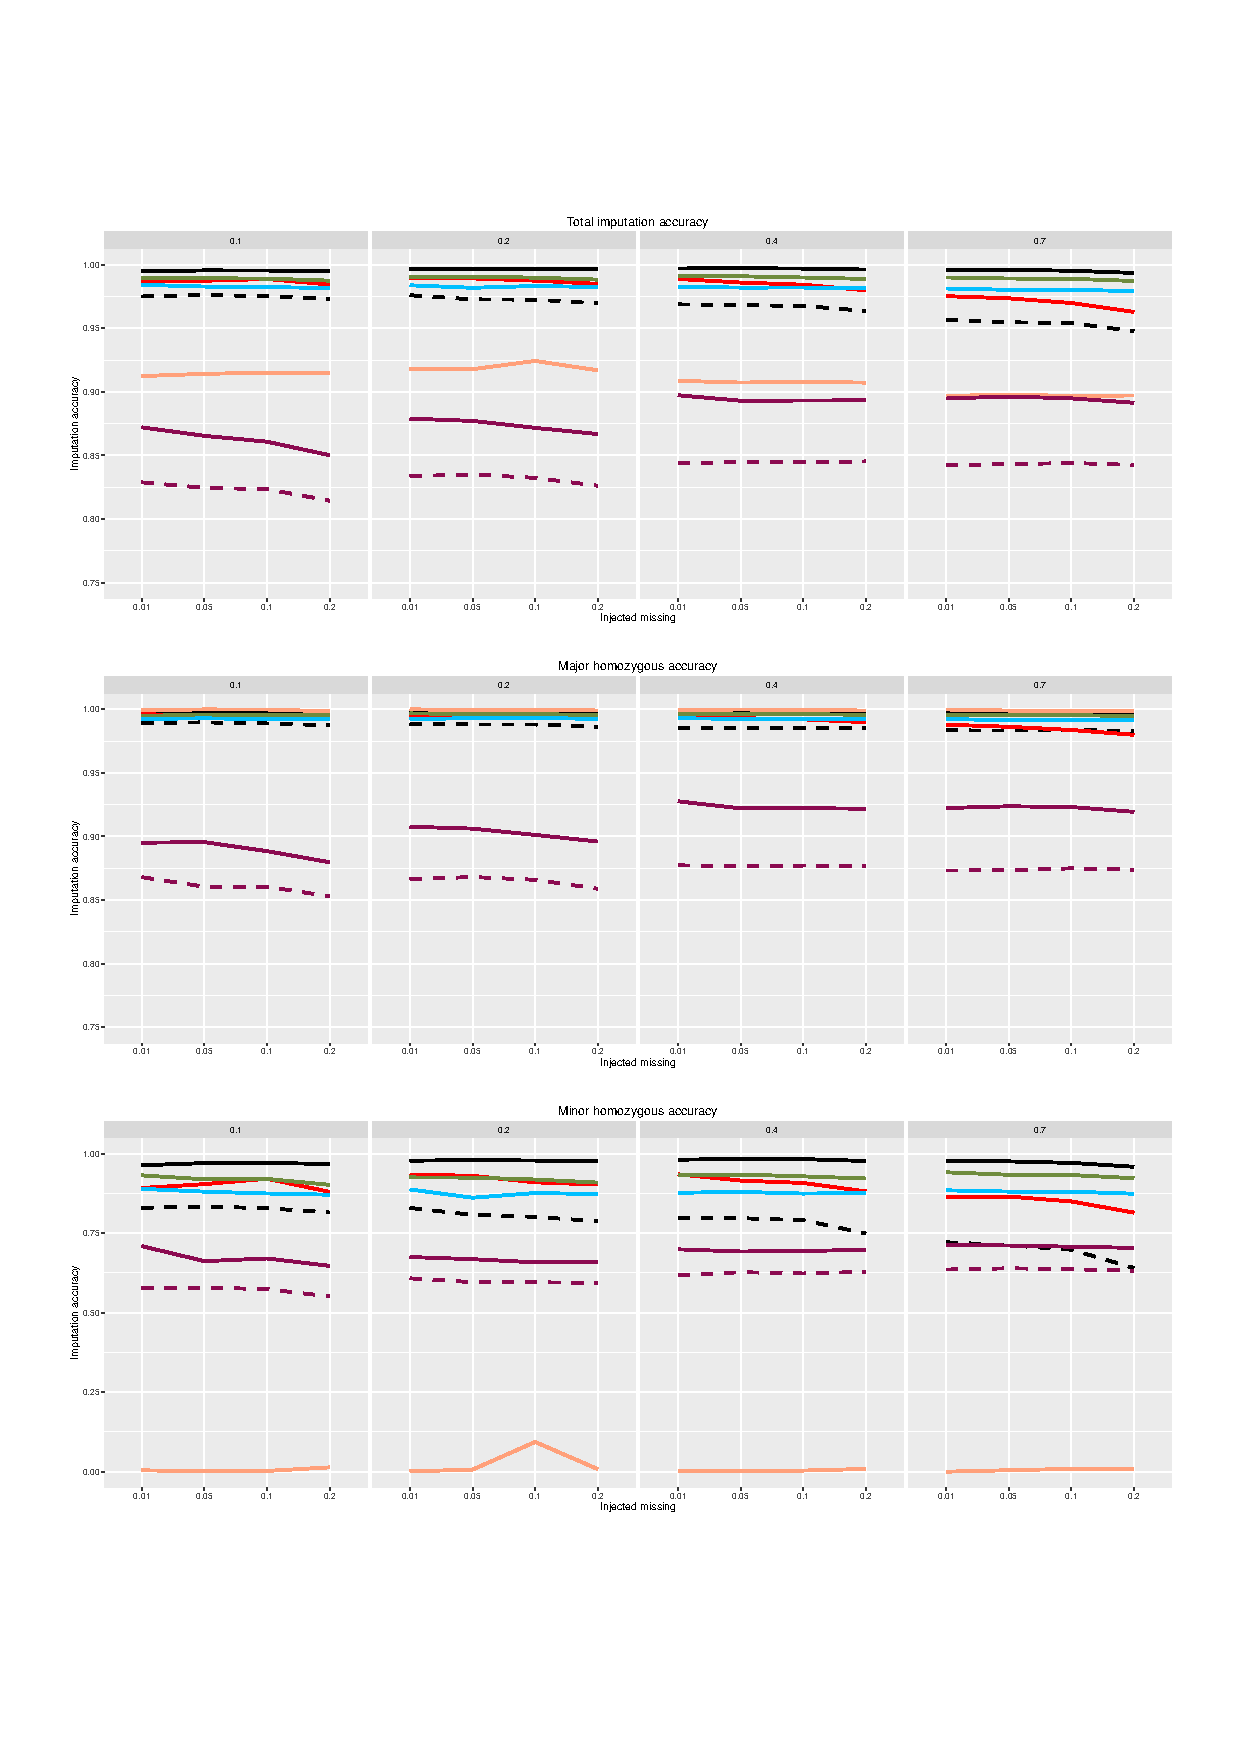
\includegraphics[width=0.95\textwidth]{figure_rice_chrom_7.pdf}\caption{
imputation accuracies overall, for the major homozygous genotype (AA) and for the minor homozygous genotype (BB) in datasets consisting of
10\%, 20\%, 40\% and 70\% allowed missing data per locus (boxes) with 1\%, 5\%, 10\% and 20\%
additional missing values artificially introduced (x-axis) for rice chromosome 7 data.
Lines colors represent the five imputation algorithms: MNI (salmon), KNNI (red), SVDI (blue), RFI (green), Beagle with ordered markers (solid black) and Beagle with unordered markers (dashed black)}\end{figure}

\begin{figure}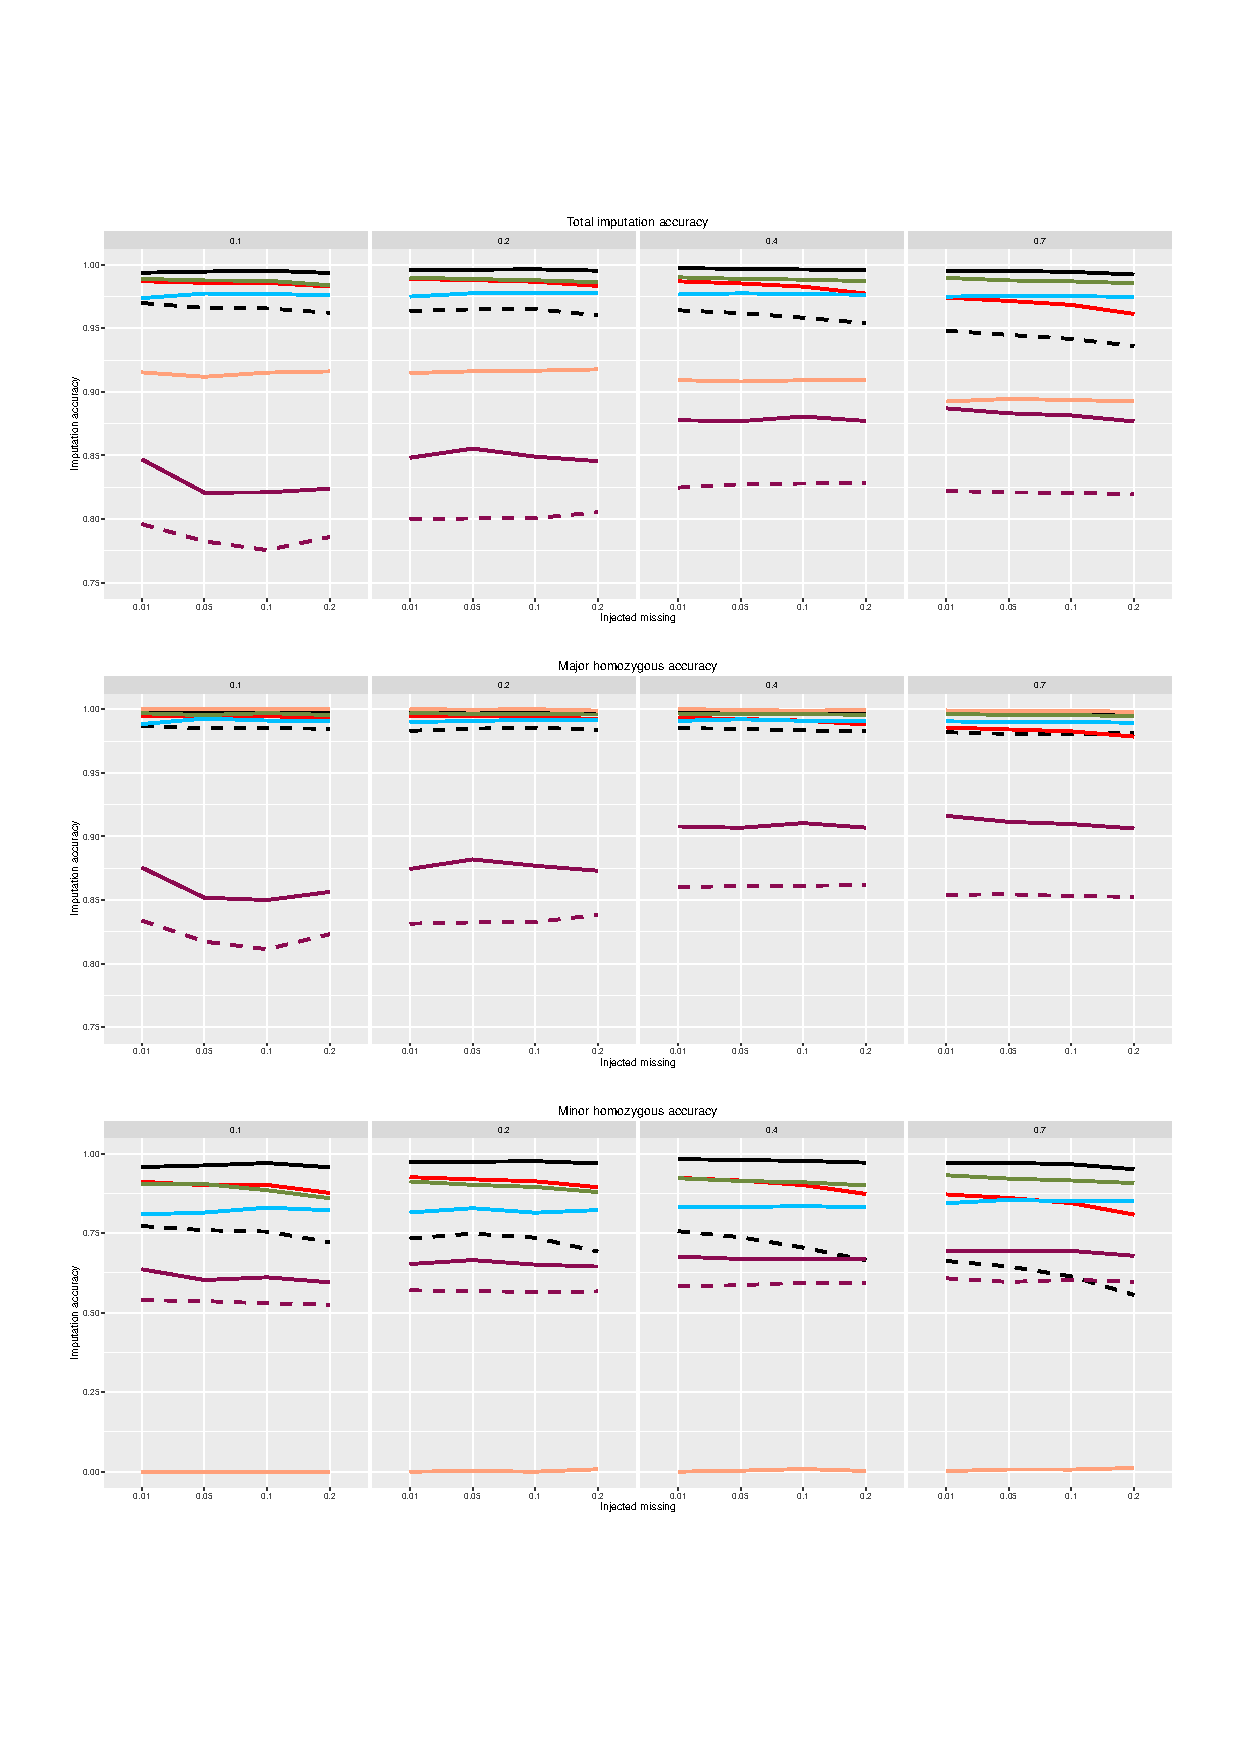
\includegraphics[width=0.95\textwidth]{figure_rice_chrom_8.pdf}\caption{
imputation accuracies overall, for the major homozygous genotype (AA) and for the minor homozygous genotype (BB) in datasets consisting of
10\%, 20\%, 40\% and 70\% allowed missing data per locus (boxes) with 1\%, 5\%, 10\% and 20\%
additional missing values artificially introduced (x-axis) for rice chromosome 8 data.
Lines colors represent the five imputation algorithms: MNI (salmon), KNNI (red), SVDI (blue), RFI (green), Beagle with ordered markers (solid black) and Beagle with unordered markers (dashed black)}\end{figure}

\begin{figure}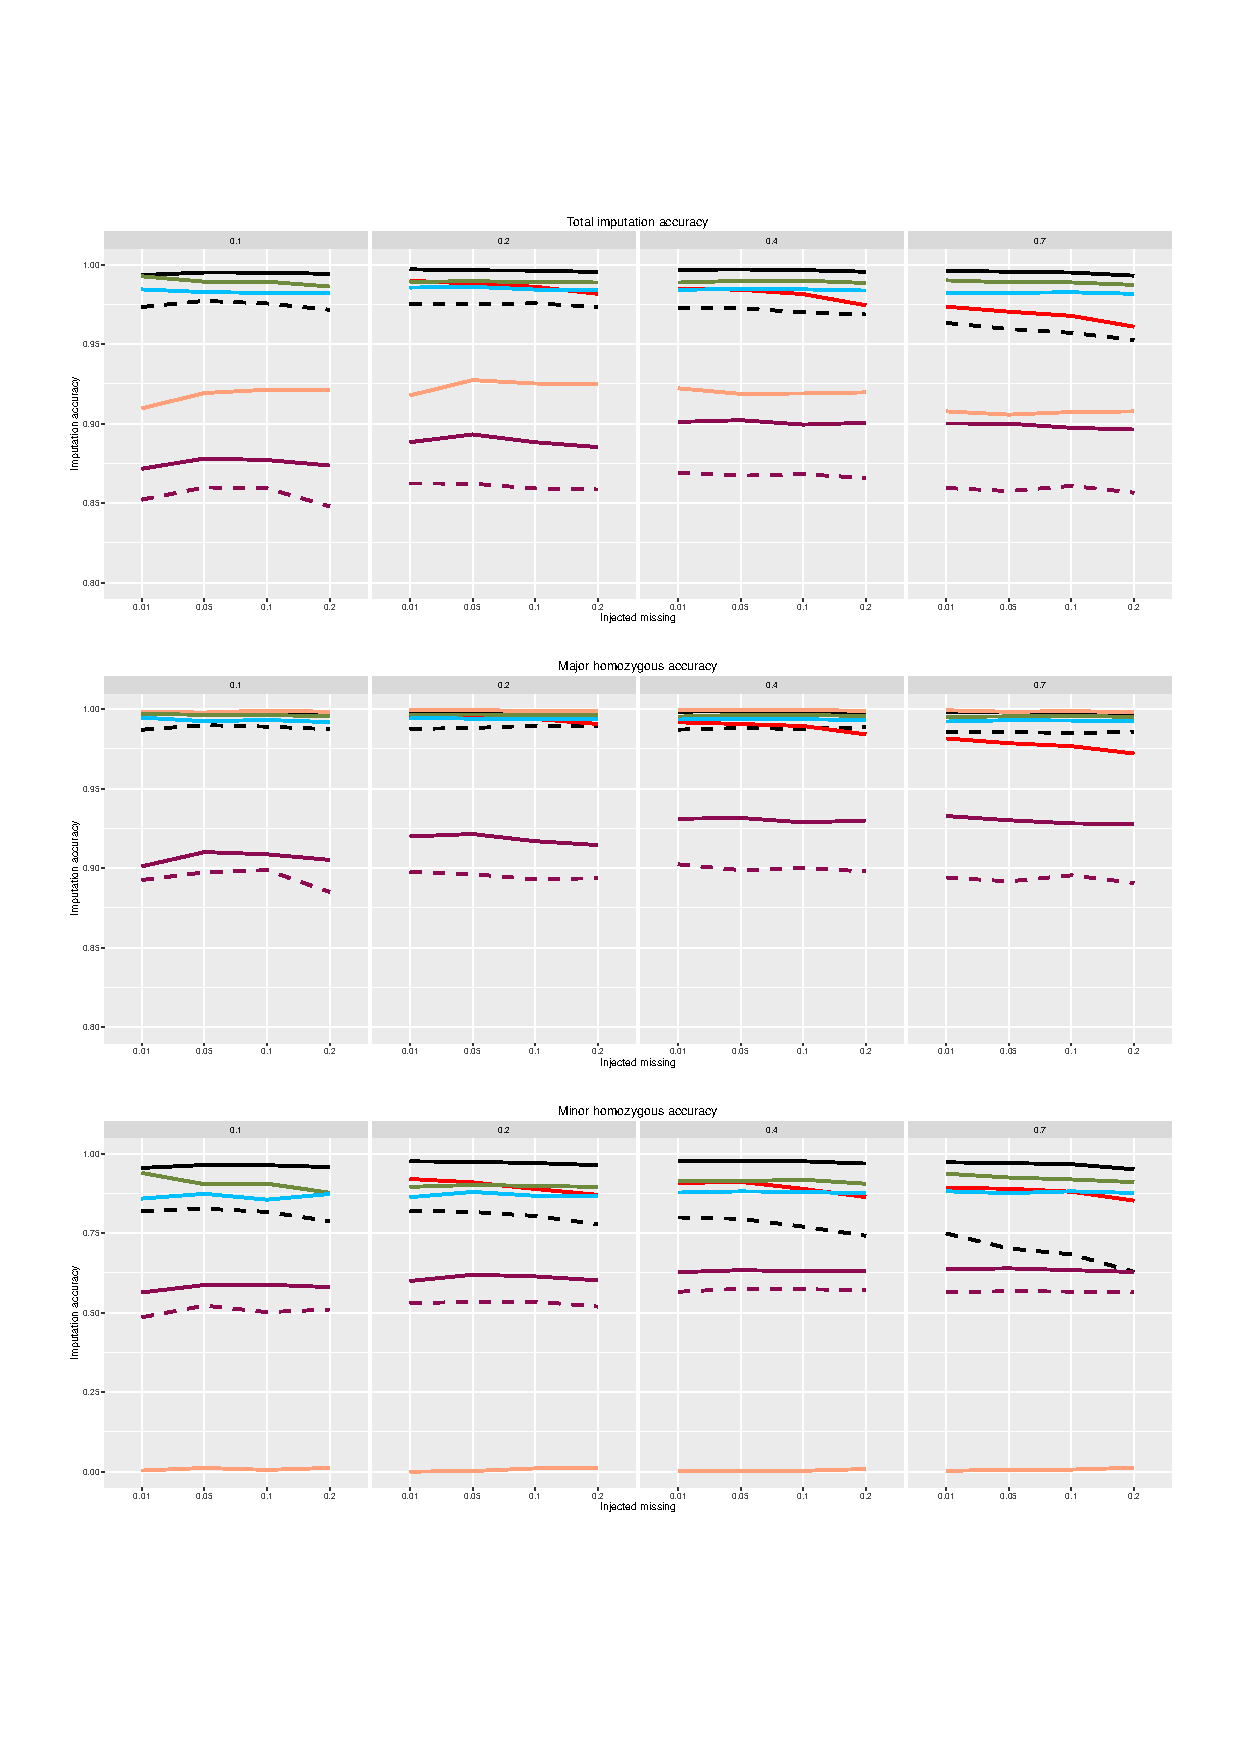
\includegraphics[width=0.95\textwidth]{figure_rice_chrom_9.pdf}\caption{
imputation accuracies overall, for the major homozygous genotype (AA) and for the minor homozygous genotype (BB) in datasets consisting of
10\%, 20\%, 40\% and 70\% allowed missing data per locus (boxes) with 1\%, 5\%, 10\% and 20\%
additional missing values artificially introduced (x-axis) for rice chromosome 9 data.
Lines colors represent the five imputation algorithms: MNI (salmon), KNNI (red), SVDI (blue), RFI (green), Beagle with ordered markers (solid black) and Beagle with unordered markers (dashed black)}\end{figure}

\begin{figure}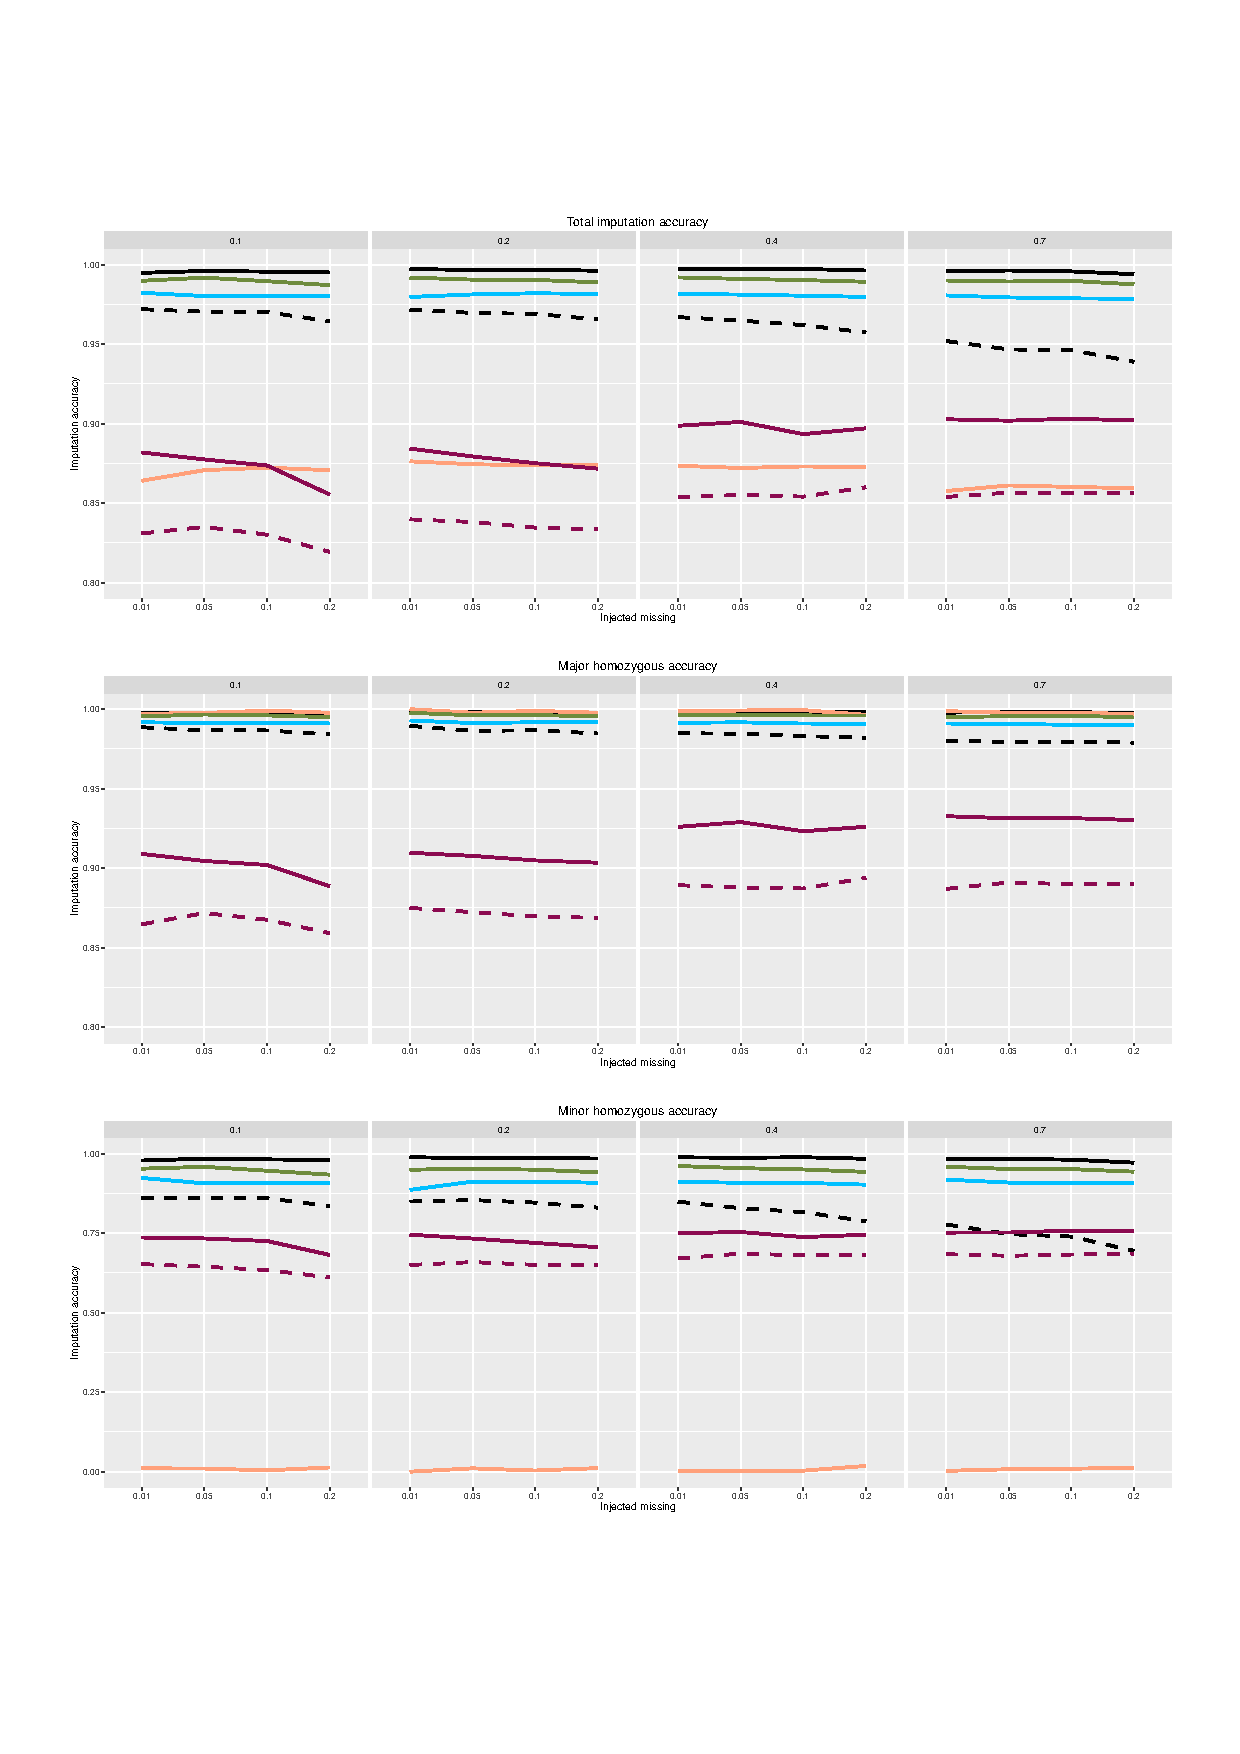
\includegraphics[width=0.95\textwidth]{figure_rice_chrom_10.pdf}\caption{
imputation accuracies overall, for the major homozygous genotype (AA) and for the minor homozygous genotype (BB) in datasets consisting of
10\%, 20\%, 40\% and 70\% allowed missing data per locus (boxes) with 1\%, 5\%, 10\% and 20\%
additional missing values artificially introduced (x-axis) for rice chromosome 10 data.
Lines colors represent the five imputation algorithms: MNI (salmon), KNNI (red), SVDI (blue), RFI (green), Beagle with ordered markers (solid black) and Beagle with unordered markers (dashed black)}\end{figure}
\begin{figure}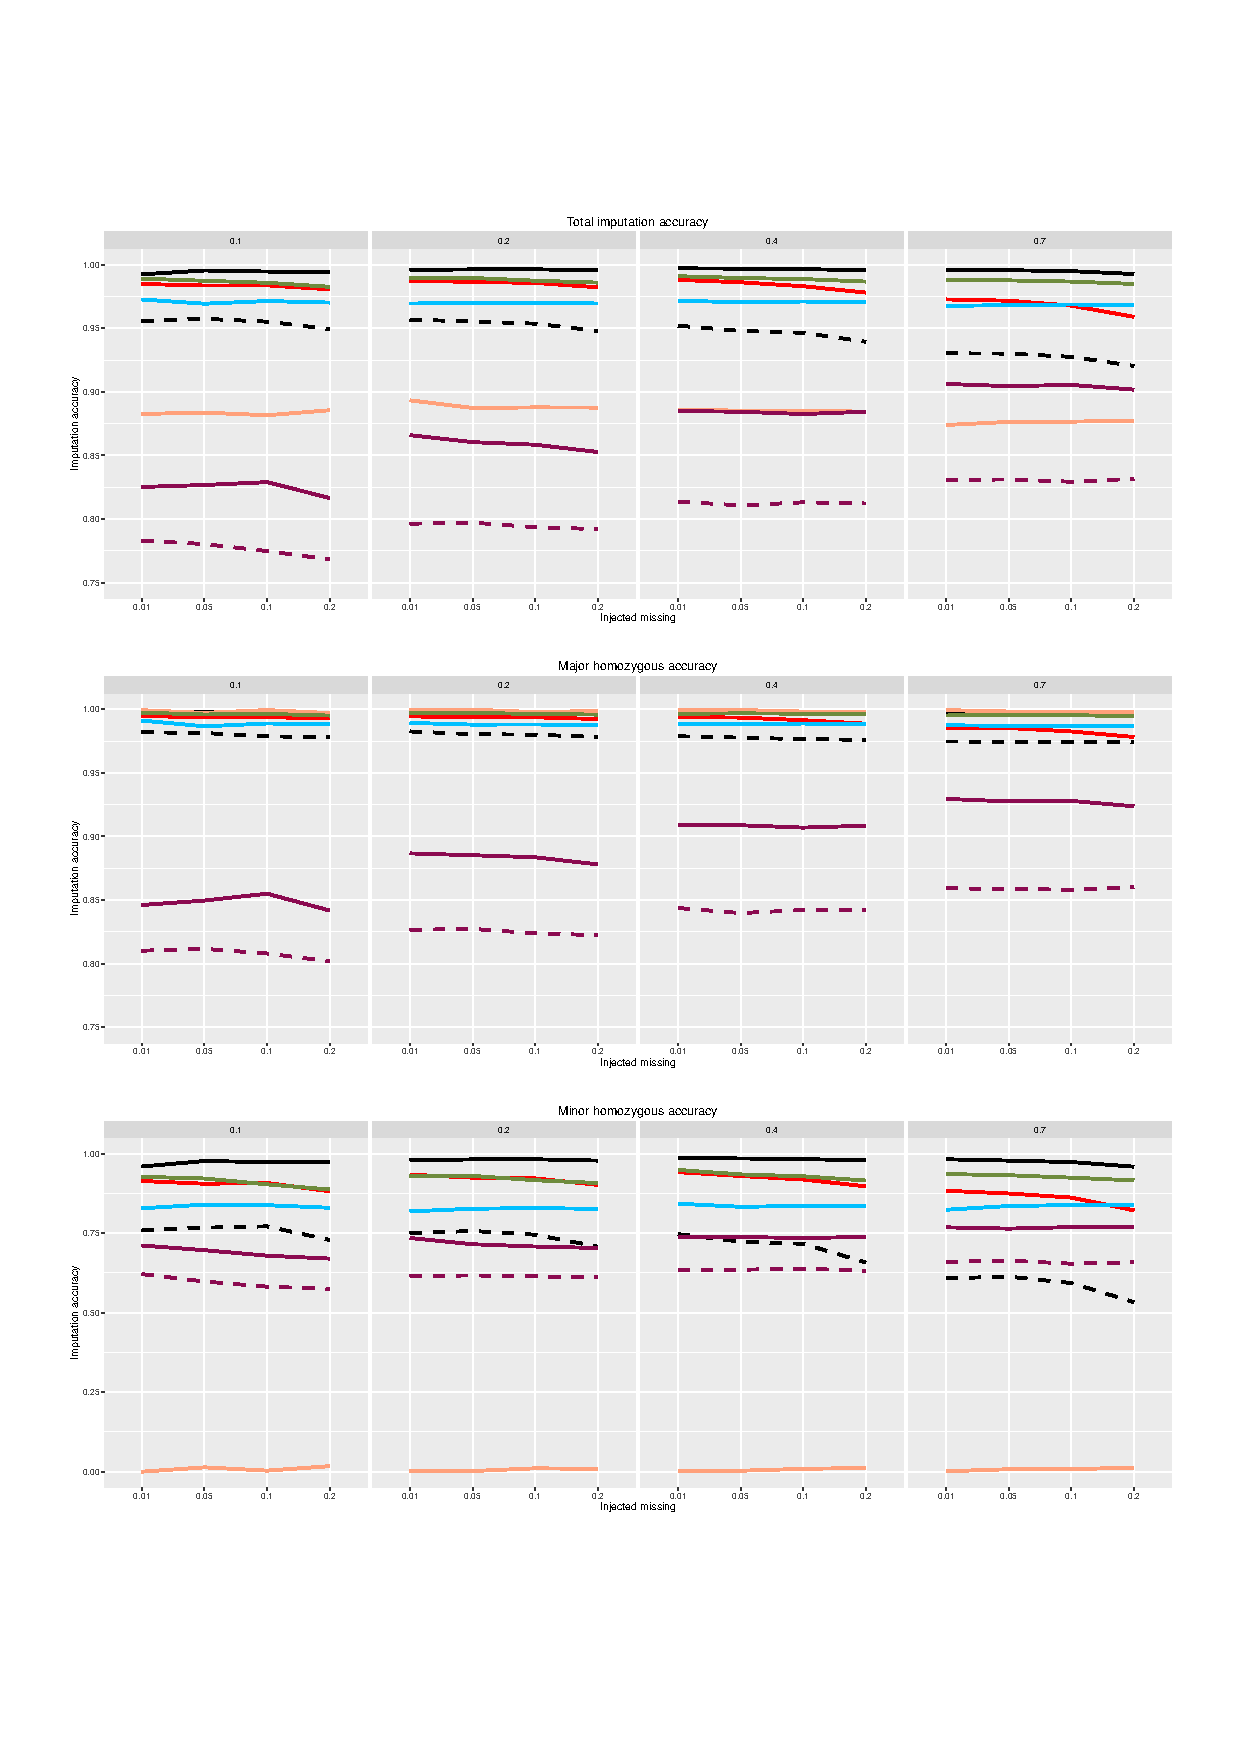
\includegraphics[width=0.95\textwidth]{figure_rice_chrom_11.pdf}\caption{
imputation accuracies overall, for the major homozygous genotype (AA) and for the minor homozygous genotype (BB) in datasets consisting of
10\%, 20\%, 40\% and 70\% allowed missing data per locus (boxes) with 1\%, 5\%, 10\% and 20\%
additional missing values artificially introduced (x-axis) for rice chromosome 11 data.
Lines colors represent the five imputation algorithms: MNI (salmon), KNNI (red), SVDI (blue), RFI (green), Beagle with ordered markers (solid black) and Beagle with unordered markers (dashed black)}\end{figure}

\begin{figure}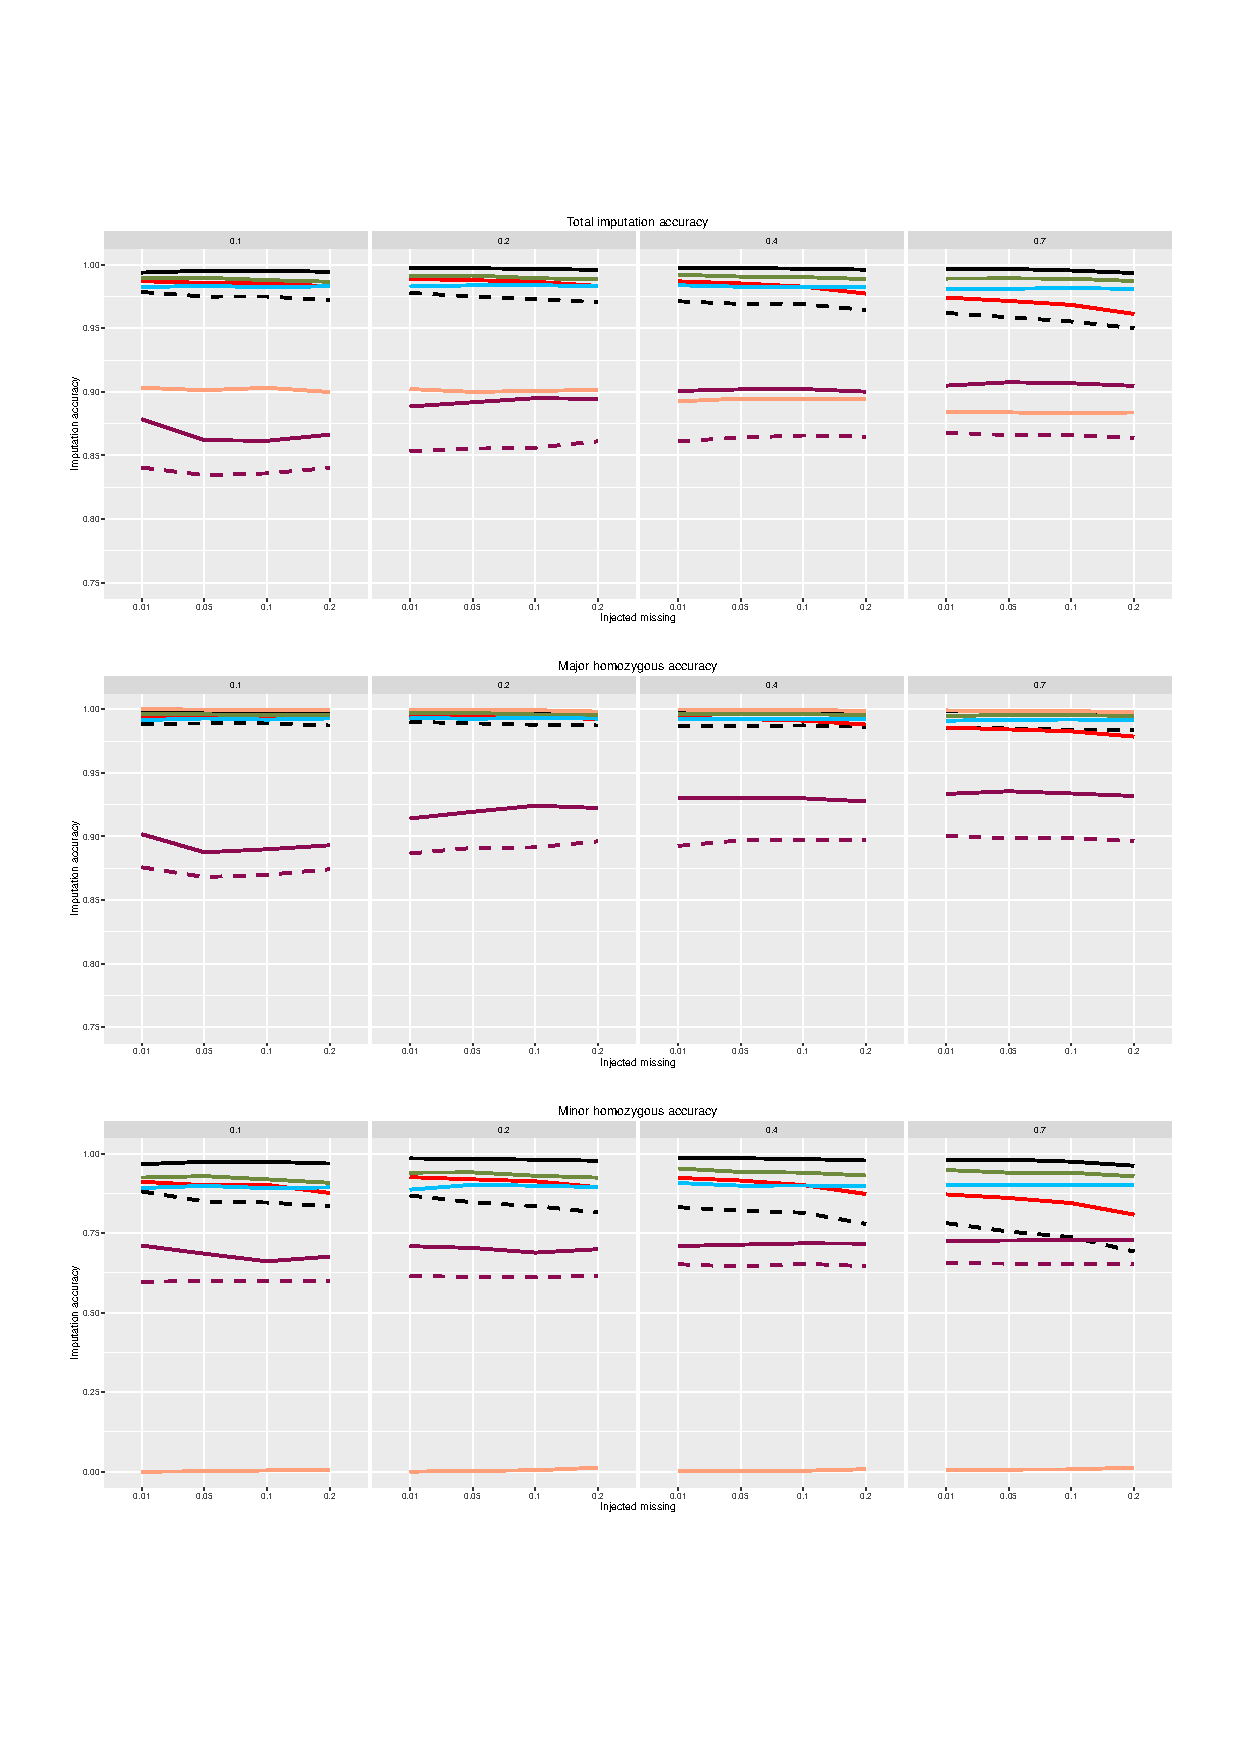
\includegraphics[width=0.95\textwidth]{figure_rice_chrom_12.pdf}\caption{
imputation accuracies overall, for the major homozygous genotype (AA) and for the minor homozygous genotype (BB) in datasets consisting of
10\%, 20\%, 40\% and 70\% allowed missing data per locus (boxes) with 1\%, 5\%, 10\% and 20\%
additional missing values artificially introduced (x-axis) for rice chromosome 12 data.
Lines colors represent the five imputation algorithms: MNI (salmon), KNNI (red), SVDI (blue), RFI (green), Beagle with ordered markers (solid black) and Beagle with unordered markers (dashed black)}\end{figure}

\begin{figure}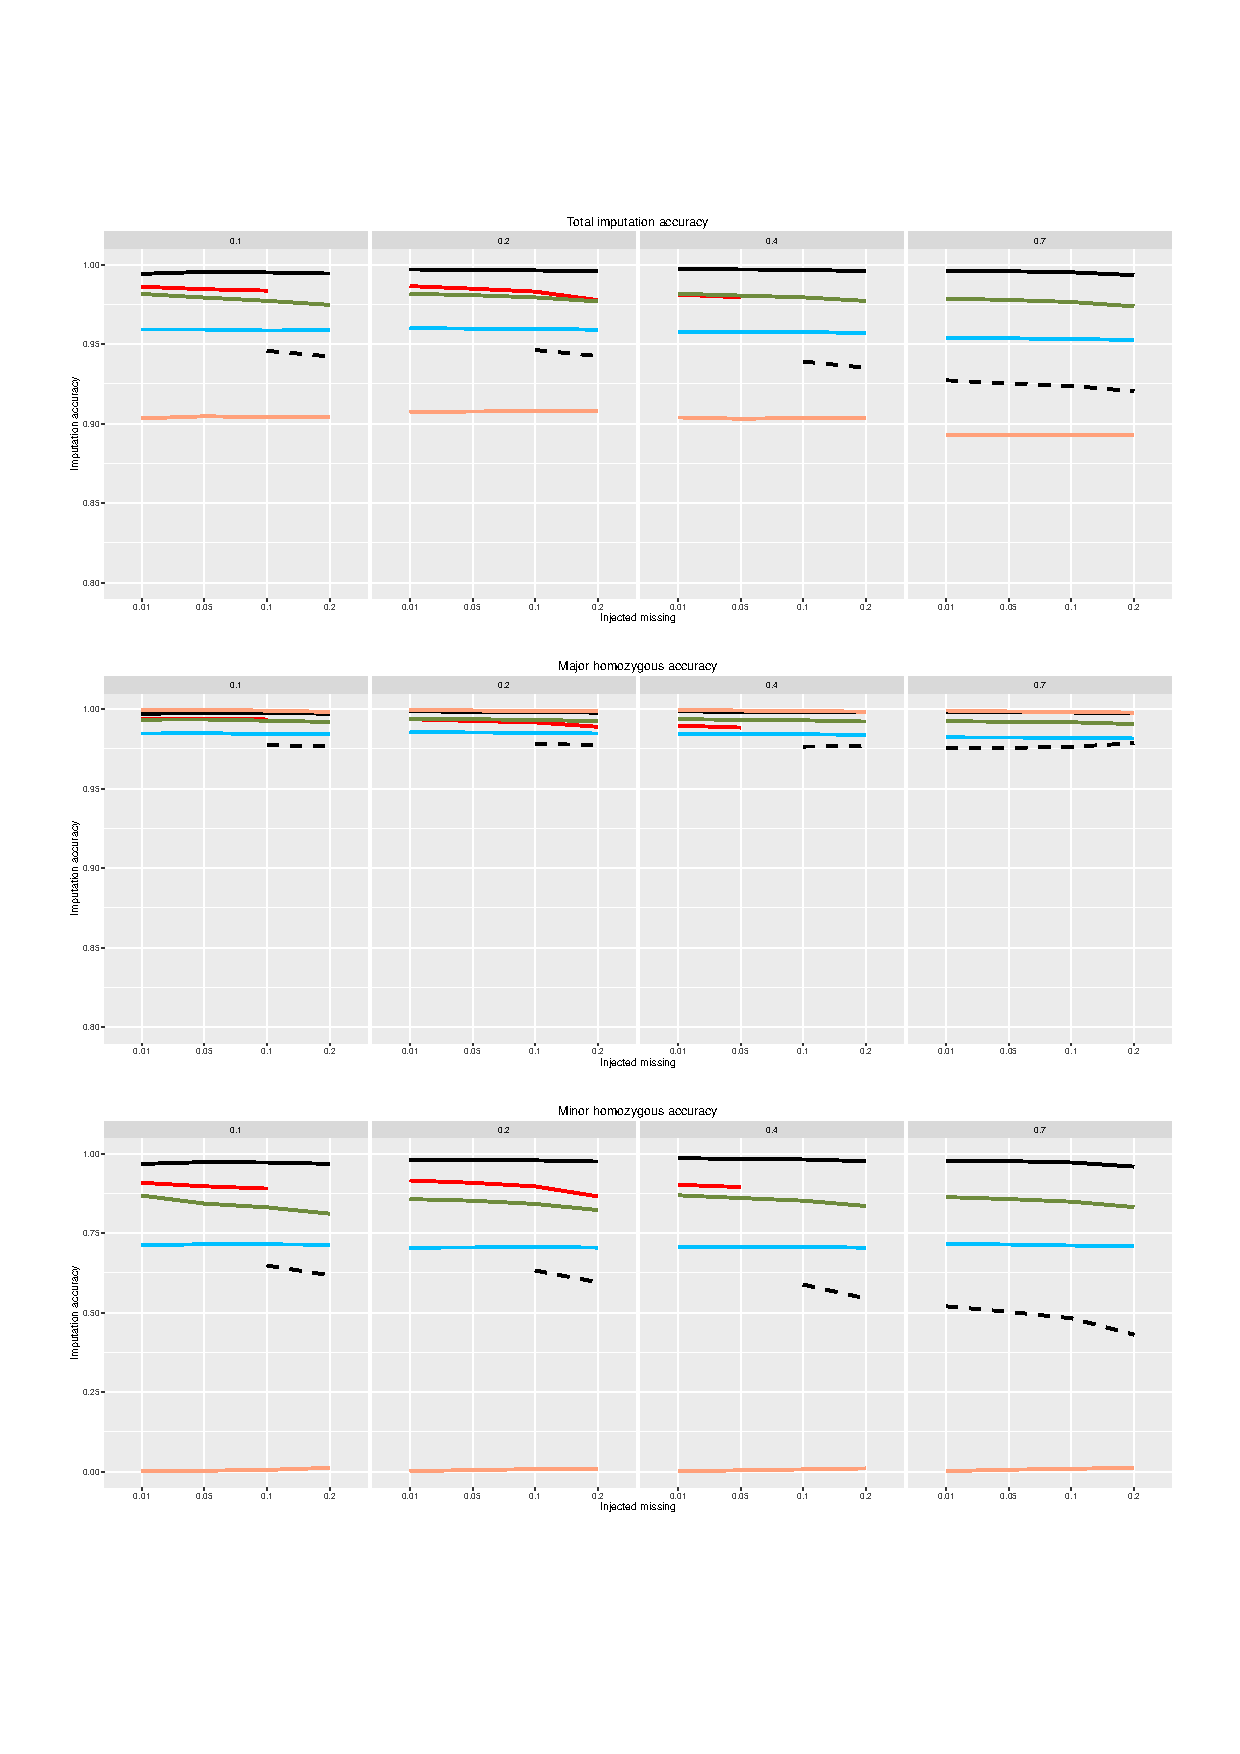
\includegraphics[width=0.95\textwidth]{figure_rice.pdf}\caption{
imputation accuracies overall, for the major homozygous genotype (AA) and for the minor homozygous genotype (BB) in datasets consisting of
10\%, 20\%, 40\% and 70\% allowed missing data per locus (boxes) with 1\%, 5\%, 10\% and 20\%
additional missing values artificially introduced (x-axis) for whole rice data set.
Lines colors represent the five imputation algorithms: MNI (salmon), KNNI (red), SVDI (blue), RFI (green), Beagle with ordered markers (solid black) and Beagle with unordered markers (dashed black)}\end{figure}













 




 

\bibliographystyle{spmpsci}      

\end{document}
